\documentclass[11pt,a4paper]{article}
\usepackage[T1]{fontenc}
\usepackage{lmodern}
\usepackage[margin=1in]{geometry}
\usepackage{microtype}
\usepackage{amsmath,amssymb,amsthm,mathtools}
\usepackage{enumitem,booktabs,graphicx}
\usepackage{needspace}
\usepackage{tikz}
\usetikzlibrary{arrows.meta,calc,positioning}
\usepackage{xcolor}
\definecolor{linkblue}{HTML}{234D73}
\usepackage[colorlinks=true,linkcolor=linkblue,citecolor=linkblue,urlcolor=linkblue]{hyperref}
\hypersetup{
  pdftitle={The Solomon--Yau least-volume theorem},
  pdfsubject={The least volume of non-equatorial minimal hypersurfaces in unit spheres},
  pdfauthor={OpenAI}
}
\newtheorem{theorem}{Theorem}[section]
\newtheorem{lemma}[theorem]{Lemma}
\newtheorem{proposition}[theorem]{Proposition}
\newtheorem{corollary}[theorem]{Corollary}
\theoremstyle{definition}
\newtheorem{definition}[theorem]{Definition}
\newtheorem{notation}[theorem]{Notation}
\theoremstyle{remark}
\newtheorem{remark}[theorem]{Remark}
\numberwithin{equation}{section}
\DeclareMathOperator{\Vol}{Vol}
\DeclareMathOperator{\Area}{Area}
\DeclareMathOperator{\ind}{ind}
\DeclareMathOperator{\spt}{spt}
\DeclareMathOperator{\dist}{dist}
\DeclareMathOperator{\tr}{tr}
\DeclareMathOperator{\diam}{diam}
\setlist[enumerate]{label=\textup{(\roman*)},leftmargin=*}
\setlist[itemize]{leftmargin=*}
\setlength{\emergencystretch}{1.5em}
\allowdisplaybreaks[1]
\widowpenalty=1000
\clubpenalty=1000
\title{The Solomon--Yau least-volume theorem}
\author{OpenAI}
\date{September 23, 2026}
\makeatletter
\renewcommand{\maketitle}{%
  \begin{center}
    {\LARGE\bfseries\@title\par}
    \vspace{0.8em}
    {\large\@author\par}
    \vspace{0.4em}
    {\@date\par}
  \end{center}
  \vspace{0.4em}
}
\makeatother

\begin{document}
\maketitle
\begin{abstract}
We prove the Solomon--Yau least-volume conjecture for minimal hypersurfaces of unit round
spheres: in every dimension \(m\ge2\), a closed connected minimal immersion
with non-totally-geodesic image has volume at least the smallest
\(m\)-dimensional minimal Clifford product. Volume is measured on the
domain, so covering multiplicities are included.
\end{abstract}

\section{Introduction}
\label{sec:introduction}

The equator is the least-volume closed minimal hypersurface of a unit
round sphere. The next volume level is a subtler question: minimality
alone gives no immediate control of topology, curvature, or singular
limits of a sequence of hypersurfaces. The natural comparison examples
are the minimal Clifford products
\[
\mathcal C_{k,m-k}
=S^k\!\left(\sqrt{\frac{k}{m}}\right)
\times S^{m-k}\!\left(\sqrt{\frac{m-k}{m}}\right)
\subset S^{m+1},\qquad 1\le k<m.
\]
The two factors have opposite principal curvatures, whose weighted sum
vanishes; these products are therefore minimal. For each integer
\(m\ge2\), set
\[
a_m=\min_{1\le k<m}\Vol_m(\mathcal C_{k,m-k}).
\]
The assertion that \(a_m\) is the first volume level above the equator
is the least-volume question in Yau's collection
\cite[Problem~31]{Yau1994}. The modern formulation in
\cite[Conjecture~1.12(ii)]{GeLi2021} calls it the Solomon--Yau conjecture.
We prove this formulation with its full immersion scope.

\begin{theorem}\label{thm:volume}
Let \(m\ge2\), let \(M^m\) be a closed connected smooth manifold, and let
\(F:M\to S^{m+1}\) be a smooth minimal immersion into the unit round sphere.
If \(F(M)\) is not totally geodesic, then
\[
\Vol\bigl(M,F^*g_{\mathrm{round}}\bigr)\ge a_m.
\]
\end{theorem}

Volume is measured on the domain, including covering multiplicities.
The theorem resolves the stated least-volume conjecture positively.
The threshold is attained by a Clifford product minimizing \(a_m\).

\subsection*{Earlier results and the geometric obstacle}

Simons' curvature identities underpin rigidity for minimal hypersurfaces
with parallel second fundamental form \cite{Simons1968}, explaining the
special role of the Clifford products. Cheng, Li, and Yau obtained a
dimension-dependent volume gap above the equator by heat-kernel
comparison \cite[Corollary~5]{ChengLiYau1984}; identifying the sharp
next level is a separate question. In dimension two, the sharp
area bound \(a_2=2\pi^2\), together with Clifford-torus rigidity, follows
from the Willmore theorem of Marques and Neves
\cite[Theorem~B and Remark~1.3]{MarquesNeves2014}.
Their canonical-family and min--max arguments connect an area comparison
to the topology of a family of surfaces. The present proof follows this
variational strategy, but the family and its topological test must work
in arbitrary hypersurface dimension.

Higher-dimensional progress includes the rotational results of Cheng,
Wei, and Zeng \cite[Theorem~1.1]{ChengWeiZeng2019}, and Viana's sharp
Clifford bound when both connected complementary regions are
antipodally invariant \cite[Theorem~1.4]{Viana2023}.
Related spectral progress includes Tang and Yan's proof that the first
positive Laplacian eigenvalue of a closed minimal isoparametric
hypersurface in the unit sphere equals its dimension
\cite[Theorem~1.1]{TangYan2013}.
Bernstein and Wang obtain near-sharp density bounds for regular minimal
cones of dimension at most six, under topological conditions on a
complementary component \cite[Theorems~1.1--1.2]{BernsteinWang2025}.
Here cone dimension is one greater than hypersurface dimension: the
density of the cone over a minimal hypersurface \(\Sigma^m\) is
\(|\Sigma|/|S^m|\). These density estimates indicate why the geometry of
cones is relevant to the volume question.

The nonembedded case has a useful independent reduction. A point with
\(q\) preimages forces domain volume at least \(q|S^m|\), as proved by
Nguyen \cite[Corollary~4.8 and Remark~4.9]{Nguyen2023} and by
Ge and Li \cite[Theorem~1.2 and Corollary~1.3]{GeLi2022}.
Since \(a_m<2|S^m|\), any counterexample to Theorem~\ref{thm:volume}
would be embedded. We give the short cone-monotonicity proof in
Proposition~\ref{prop:immersion-reduction}, retaining tangent and
coincident sheets. The more recent general embedded-hypersurface bounds of Ge and Li
\cite[Theorems~1.4 and 1.6]{GeLi2026II} remain below the sharp Clifford
threshold, which their Conjecture~1.3 still poses as the target.

After this reduction, the central difficulty is to minimize area among
non-equatorial counterexamples and then decrease that minimum.
Ordinary varifold compactness may produce singular limits, while a
variational construction must retain enough topology to avoid collapsing
to an equator. We address these two requirements together: a detecting
family gives a uniform gap above the equator, and a dimension induction
rules out singularities below the Clifford threshold.

\subsection*{Curvature, index, and the variational family}

The first construction controls both signs of the principal curvatures.
For a closed embedded non-equatorial minimal hypersurface \(\Sigma^m\),
with second fundamental form \(A\), a two-point maximum compares the
normal at one point with every other point of \(\Sigma\).
The reflection calculation is related to the two-point methods in
\cite[Section~2]{Brendle2013} and \cite[Section~2]{AHLW2015}.
We prove the required static differential
inequality directly, including diagonal contacts and repeated principal
curvatures. A smooth upper-test comparison then gives
\[
\int_\Sigma |A|^2\ge m|\Sigma|.
\]
This proves the lower-bound assertion of Perdomo's average-curvature
conjecture \cite[Conjecture~1.5]{GeLi2021}.
Combining it with the conformal and spectral mechanism of
\cite[Theorem~3.1]{Perdomo2004}, and keeping track of equality in each
spectral inequality, shows that index \(m+3\) forces a Clifford product
(Proposition~\ref{prop:index-rigidity}). A counterexample must
therefore have a further negative direction for area.

The average-curvature inequality and this embedded index classification
also appear in Nifa's recent preprint
\cite[Theorem~1.1 and Corollary~7.3]{Nifa2026}, which proves a stronger
Schr\"odinger quadratic-form inequality. His construction uses the sum
of two tangent-ball curvatures and a weak supersolution. Here a two-sided
maximum and a smooth Poisson comparison suffice for the integrated
bound. We give the curvature and index arguments in full, independently
of the volume comparison that follows.

The second construction turns that direction into a strict area
improvement. Form the Euclidean cone over \(\Sigma\), take its signed
distance function, and regard the graph as a hypersurface in a space
with one time coordinate. Lorentz boosts preserve the difference
between squared spatial length and squared time. Intersecting the
transformed graph with the unit spatial sphere produces level sets
whose areas are controlled on the fixed source \(\Sigma\).
At each closest-point contact, minimality makes a nonnegative Jacobian
matrix have fixed trace; its determinant bounds the area of the level.
This estimate works even when closest points are not unique.

The boost parameters and the level parameter give a family on
\(\mathbb{RP}^{m+3}\). Its boundary cycles have area at most
\(|\Sigma|\), and its fillings change to their complements around the
projective generator. The associated degree-one cohomology class has
nonzero \((m+3)\)-rd power. This is the topological detection used in
Section~\ref{sec:minmax}; it replaces a topology assumption on
\(\Sigma\) itself. The original hypersurface is the unique area
maximum, with a uniform gap away from its central parameter.
Its extra index direction removes that maximum while preserving the
detection and the absence of mass concentration
(Proposition~\ref{prop:lorentz-family}).

\subsection*{Compactness and the final induction}

Detection forces every such family to contain a boundary of a
half-volume region with zero centroid. Spherical isoperimetry and its
hemisphere equality case give a uniform area threshold
\(\gamma_m>|S^m|\) for these boundaries
(Lemma~\ref{lem:detection-gap}). The min--max theorem therefore produces
stationary integral varifolds above the equator, even after the
strict deformation.

The volume proof proceeds by induction on \(m\). Assuming only the
lower-dimensional volume statements, Section~\ref{sec:cones} proves
regularity for the subthreshold limits arising both from minimizing
sequences and from min--max. The mechanism is radial splitting:
tangents at nonzero points of a Euclidean cone split off a line,
reducing their classification to a smaller cone dimension. This gives
smooth connected links of multiplicity one without applying the
unknown dimension-\(m\) volume theorem to those links.

Compactness therefore attains a least counterexample of area \(H\),
with \(\gamma_m\le H<a_m\). Its index exceeds \(m+3\), so the deformed
family has maximum area strictly below \(H\). Min--max produces a
varifold of mass in \([\gamma_m,H)\), and the same regularity argument
makes it a smooth connected multiplicity-one hypersurface. Its mass
is above the equator and below \(H\): it is a smaller counterexample,
the desired contradiction. The induction starts at \(m=2\), with
no lower-dimensional volume hypothesis.

Section~\ref{sec:preliminaries} establishes the volume normalization and
immersion reduction. Section~\ref{sec:index} proves curvature and index
rigidity. Section~\ref{sec:minmax} establishes detection and the precise
min--max interface before Section~\ref{sec:family} constructs and deforms
the Lorentz-distance family. Section~\ref{sec:cones} proves the cone
induction and exact attainment, and Section~\ref{sec:conclusion}
completes the proof.

\section{Normalization and the immersion reduction}
\label{sec:preliminaries}

All spheres have radius one unless a radius is displayed. We write
\(\sigma_j=\Vol_j(S^j)\) and \(\omega_j=\Vol_j(B^j_1)\), so
\(\sigma_{j-1}=j\omega_j\). For an embedded hypersurface \(\Sigma\),
\(|\Sigma|\) denotes its induced \(m\)-volume. The word closed means
compact without boundary.

The Laplacian is \(\Delta=\operatorname{div}\nabla\). For a two-sided
minimal hypersurface in a sphere, \(x\) is the position vector, \(N\) a
global unit normal, \(A=-dN\) the shape operator, and \(P=|A|^2\).
The Morse index counts the positive eigenvalues, with multiplicity, of
\[
L=\Delta+m+P;
\]
equivalently it is the dimension of a maximal negative subspace for
the area second variation \(-\int_\Sigma uLu\).

\begin{lemma}\label{lem:clifford-ratios}
The numbers \(\vartheta_m=a_m/\sigma_m\) strictly decrease for
integers \(m\ge2\). Moreover,
\[
\vartheta_2=\frac{\pi}{2}<2,
\qquad
\vartheta_4\le\frac32.
\]
Consequently \(a_m<2\sigma_m\) for every \(m\ge2\), and
\(\vartheta_m\le3/2\) for every \(m\ge4\).
\end{lemma}

\begin{proof}
For \(k+l=m\), the product has volume
\[
\sigma_k\sigma_l
\left(\frac{k}{m}\right)^{k/2}
\left(\frac{l}{m}\right)^{l/2}.
\]
Define, for real \(j>0\),
\[
d_j=\sigma_j\left(\frac{j}{2\pi e}\right)^{j/2},
\qquad
\sigma_j=\frac{2\pi^{(j+1)/2}}{\Gamma((j+1)/2)}.
\]
The ratio of the product volume to \(\sigma_m\) is \(d_kd_l/d_{k+l}\).
The usual series for the logarithmic derivatives of \(\Gamma\) gives
\[
\frac{d^2}{dj^2}\log d_j
=\frac1{2j}
-\frac14\sum_{i=0}^{\infty}
\left(i+\frac{j+1}{2}\right)^{-2}>0.
\]
Indeed, strict convexity of \(t\mapsto(t+j/2)^{-2}\) implies
\[
\sum_{i=0}^{\infty}\left(i+\frac{j+1}{2}\right)^{-2}
<
\int_0^\infty(t+j/2)^{-2}\,dt
=\frac2j.
\]
Thus, with \(k>0\) fixed, the derivative in \(l\) of
\(\log(d_kd_l/d_{k+l})\) is negative. Increase the second entry of a
minimizing pair for \(m\) by one to obtain a strictly smaller competitor
for \(\vartheta_{m+1}\). This proves the strict decrease. The stated
values follow from \(k=l=1\) and \(k=l=2\), respectively.
\end{proof}

For a \(d\)-dimensional Euclidean varifold \(V\), its density at \(z\),
when it exists, is
\[
\Theta(V,z)=\lim_{\rho\downarrow0}
\frac{\|V\|(B_\rho(z))}{\omega_d\rho^d}.
\]
Here \(\|V\|\) is its weight measure. We use stationary integral
varifolds with their full integer multiplicities. In particular,
coincident sheets add their masses.

The following multiplicity estimate is due to Nguyen
\cite[Corollary~4.8]{Nguyen2023} and Ge--Li
\cite[Theorem~1.2]{GeLi2022}. We include its cone-monotonicity proof to
make the treatment of source multiplicity explicit.

\begin{proposition}[Immersion reduction]\label{prop:immersion-reduction}
Let \(F:M^m\to S^{m+1}\) be a smooth minimal immersion of a closed
manifold, with \(m\ge2\). If some image point has \(q\) preimages, then
\[
\Vol\bigl(M,F^*g_{\mathrm{round}}\bigr)\ge q\sigma_m.
\]
In particular, every immersion violating the bound in
Theorem~\ref{thm:volume} is an embedding.
\end{proposition}

\begin{proof}
Push forward the parametrized Euclidean cone
\[
(0,\infty)\times M\longrightarrow\mathbb R^{m+2},
\qquad (r,z)\longmapsto rF(z),
\]
with measure \(r^m\,dr\,d\mathrm{vol}_M\). This gives an integral
\((m+1)\)-varifold \(\mathcal C_F\), extended with zero mass at the
origin. Minimality of \(F\) makes it stationary away from the origin.
The boundary term for first variation after truncation at \(r=\epsilon\)
is \(O(\epsilon^m)\); it tends to zero. Thus \(\mathcal C_F\) is
stationary in all of Euclidean space. The corresponding calculation
for general spherical varifolds is given in Lemma~\ref{lem:cone-operation}.

Its centered ball masses are exactly
\[
\|\mathcal C_F\|(B_R(0))
=\frac{R^{m+1}}{m+1}
\Vol\bigl(M,F^*g_{\mathrm{round}}\bigr),
\]
and hence
\[
\Theta(\mathcal C_F,0)
=\frac{\Vol(M,F^*g_{\mathrm{round}})}{\sigma_m}.
\]
Every fiber of a compact immersion is finite: it is compact and its
points are isolated by local embedding neighborhoods. At a nonzero
cone point over an image point with \(q\) preimages, these neighborhoods
give \(q\) smooth local sheets, each of density one. Therefore the density
there is \(q\), even when tangent planes agree or sheets coincide.

For a fixed Euclidean center \(z\), the inclusions
\[
B_{R-|z|}(0)\subset B_R(z)\subset B_{R+|z|}(0)
\]
show that the large-radius mass ratio has limit
\(\Theta(\mathcal C_F,0)\). Stationary monotonicity centered at the
chosen nonzero point consequently gives
\[
q\le \Theta(\mathcal C_F,0).
\]
This proves the inequality. If \(F\) is not injective, take \(q\ge2\)
and use Lemma~\ref{lem:clifford-ratios}. Finally, an injective immersion
from a compact manifold is an embedding.
\end{proof}

\begin{remark}\label{rem:preliminaries-multiplicity}
The preceding argument counts preimages at the actual point; it does
not require transverse self-intersections. On a regular image patch,
the number of coincident sheets is the usual local covering
multiplicity. Distinct minimal sheet germs are analytic and meet in a
set of hypersurface measure zero unless they agree. Thus the generic
multiplicity on such patches also has its ordinary covering
interpretation. In particular, replacing a minimal embedding by a
finite covering multiplies the measured volume by its degree.
\end{remark}

\begin{lemma}\label{lem:fullness}
A closed connected embedded non-equatorial minimal hypersurface
\(\Sigma^m\subset S^{m+1}\) is two-sided and full, meaning that its
position vectors span \(\mathbb R^{m+2}\). It is real analytic, and
\[
\int_\Sigma x=0.
\]
For every nonzero constant vector \(a\), the coordinate function
\(\langle a,x\rangle\) is nontrivial and its zero set has
\(m\)-dimensional measure zero.
\end{lemma}

\begin{proof}
A closed embedded hypersurface in a sphere separates it into two
regions and has a global unit normal. If its image were contained in
a linear hyperplane, it would be an open and closed subset of the
corresponding great sphere, by equality of dimensions. Connectedness
and compactness would make the image that great sphere. This proves
fullness.

The coordinate equation \(\Delta x=-mx\) gives the integral identity.
In analytic ambient coordinates, a minimal hypersurface is locally an
analytic graph by analytic regularity for the minimal graph equation
\cite[Theorem~1.1]{Blatt2024}.
Thus its coordinate functions are analytic. Fullness makes each
\(\langle a,x\rangle\), \(a\ne0\), nontrivial, and a nontrivial analytic
function on a connected manifold has a zero set of measure zero
\cite[Proposition~0]{Mityagin2015}.
\end{proof}

\section{Average curvature and index rigidity}\label{sec:index}

Throughout this section, $\Sigma^m\subset S^{m+1}$ is a smooth, closed,
connected, embedded minimal hypersurface, $m\ge2$, which is not totally
geodesic.  Write $x$ for its position vector, $N$ for a global unit normal,
$A=-dN$ for its shape operator, and $P=|A|^2$.  Integrals use the induced
volume measure $dV$; set $V_\Sigma=\Vol_m(\Sigma)$.  The inequality
\[
  \int_\Sigma P\,dV\ge mV_\Sigma
\]
is the inequality part of Perdomo's conjecture, as formulated in
\cite[Conjecture~1.5]{GeLi2021}.  We prove it by a two-sided curvature
maximum.  Combining it with the conformal and spectral argument of
\cite[Theorem~3.1]{Perdomo2004} then gives the index rigidity needed below.
We include that argument, in particular its pointwise equality step.

With $\Delta=\operatorname{div}\nabla$, the minimal hypersurface identities
are
\begin{equation}\label{eq:index-geometric-identities}
 \Delta x=-mx,\qquad \Delta N=-PN,\qquad
 \Delta A=(m-P)A,\qquad
 \frac12\Delta P=|\nabla A|^2+(m-P)P.
\end{equation}
Here the Laplacian of $A$ is the rough tensor Laplacian.  We also use
$\tr A=0$ and the Codazzi identity: $\nabla A$, viewed as a covariant
three-tensor, is symmetric.  The last two formulas are the hypersurface
case of Simons' identity
\cite[Theorem~5.3.1, equation~(5.3.2)]{Simons1968}.

\subsection{A two-sided curvature maximum}

Define
\begin{equation}\label{eq:index-mu}
 \mu(x)=\sup_{\substack{y\in\Sigma\\y\ne x}}
 \frac{|\langle N(x),y\rangle|}{1-\langle x,y\rangle}.
\end{equation}
Embeddedness makes the denominator positive away from the diagonal.
The absolute value controls both signs of the principal curvatures.
The reflection used below appears in Brendle's two-point argument
\cite[Section~2]{Brendle2013} and in curvature estimates for hypersurface
flows \cite[Section~2]{AHLW2015}. The diagonal and distinct-point contact
calculations are also closely related to
\cite[Lemma~3.5 and Proposition~4.1]{Nifa2026}.
Using the sum of the two one-sided tangent-ball curvature functions,
Nifa obtains a stronger quadratic-form inequality and derives both the
average-curvature bound and the embedded least-index classification
\cite[Theorem~1.1 and Corollary~7.3]{Nifa2026}.
For the integrated estimate needed here, the absolute maximum in
\eqref{eq:index-mu} suffices. We prove its differential inequality directly.

Rather than differentiate the maximum, we estimate smooth upper tests.
The logarithmic form of the estimate will allow comparison with a Poisson
potential, forcing the mean of $m-P$ to be nonpositive.

\begin{lemma}[Upper tests for the curvature maximum]
\label{lem:index-upper-tests}
The function $\mu$ in \eqref{eq:index-mu} is finite, continuous, and strictly
positive.  If a smooth positive function $\phi$ satisfies $\phi\ge\mu$ in
a neighborhood of $x$ and $\phi(x)=\mu(x)$, then
\begin{equation}\label{eq:index-log-test}
 \Delta\log\phi(x)\ge m-P(x).
\end{equation}
\end{lemma}

\begin{proof}
We first describe the possible contacts.  Let
$\gamma(t)=\exp_x(tv)$, where $v\in T_x\Sigma$ is a unit vector, and regard
$\gamma$ as a curve in $\mathbb R^{m+2}$.  The ambient differentiation
formulas give
\begin{align}
 \langle N(x),\gamma(t)\rangle
   &=\frac{t^2}{2}A_x(v,v)
     +\frac{t^3}{6}(\nabla_vA)_x(v,v)+O(t^4),
       \label{eq:index-contact-numerator}\\
 1-\langle x,\gamma(t)\rangle
   &=\frac{t^2}{2}+O(t^4).
       \label{eq:index-contact-denominator}
\end{align}
For example, $\gamma''(0)=-x+A_x(v,v)N(x)$, while
$\langle x,\gamma'''(0)\rangle=0$.  Compactness makes these expansions
uniform on the unit tangent bundle for sufficiently small $|t|$.
Consequently, adjoining unit tangent directions at the diagonal extends
the quotient continuously, with values $|A_x(v,v)|$.

For completeness, this extension also gives continuity when the base
point varies.  If $x_j\to x$ and nearly maximizing points $y_j$ stay away
from $x$, a convergent subsequence gives an ordinary distinct-point
contact.  If $y_j\to x$, write
$y_j=\exp_{x_j}(t_jv_j)$ and take a convergent subsequence of unit tangent
directions.  The uniform expansions show that its limiting quotient is
at most $\mu(x)$.  This proves upper semicontinuity.  Holding fixed any
$y\ne x$ whose quotient is within $\varepsilon$ of $\mu(x)$ proves lower
semicontinuity, after letting $\varepsilon\downarrow0$.  The same
compactness argument proves finiteness and shows that a maximum is
realized either by distinct points or by a tangent direction.  If
$\mu(x)=0$, the entire hypersurface lies in $N(x)^\perp$, contrary to
fullness from Lemma~\ref{lem:fullness}.  Thus $\mu>0$.

Fix an upper test $\phi$ at $x$.  At a realizing contact, choose the sign
of $N$ to make the signed quotient positive, and change the sign of $A$
at the same time.  This choice is held fixed in a neighborhood.  It
requires no continuous choice of maximizing sign: for either fixed sign
and for every nearby $x'$ and every $y'\ne x'$,
\begin{equation}\label{eq:index-fixed-sign}
 \frac{\langle N(x'),y'\rangle}{1-\langle x',y'\rangle}
 \le\mu(x')\le\phi(x').
\end{equation}
Choose a principal orthonormal basis $e_1,\ldots,e_m$ at $x$, and write
$Ae_i=\lambda_i e_i$.  The diagonal limits give
\begin{equation}\label{eq:index-two-sided-eigenvalues}
 -\phi(x)\le\lambda_i\le\phi(x)\qquad(1\le i\le m).
\end{equation}
We shall prove the stronger inequality
\begin{equation}\label{eq:index-gradient-test}
 \Delta\phi+(P-m)\phi
 \ge 2\sum_{\lambda_i<\phi}
             \frac{\phi_i^2}{\phi-\lambda_i}
 \ge\frac{|\nabla\phi|^2}{\phi}
 \quad\text{at }x,
\end{equation}
where $\phi_i=d\phi(e_i)$ and every component with $\lambda_i=\phi$
will be shown to vanish.

\smallskip
\noindent\emph{Distinct-point contact.}
Suppose $y\ne x$ realizes the maximum with the chosen sign.  On the
product of a neighborhood of $x$ with $\Sigma$, set
\[
 Z(x',y')=\phi(x')\bigl(1-\langle x',y'\rangle\bigr)
                  -\langle N(x'),y'\rangle.
\]
By \eqref{eq:index-fixed-sign}, $Z\ge0$ and $Z(x,y)=0$.  Write
$c=\langle x,y\rangle$, $s=1-c>0$, and $d_i=\langle e_i,y\rangle$.
The first derivatives at the minimum give
\begin{equation}\label{eq:index-distinct-first}
 s\phi_i=(\phi-\lambda_i)d_i.
\end{equation}
Reflection across the hyperplane perpendicular to $x-y$ sends $x$ to
$y$, and sends $N(x)$ to
\[
 n_y=N(x)+\phi(x-y).
\]
Indeed $\langle N(x),y\rangle=\phi s$, so this vector is perpendicular to
$y$ and has length one.  The $y$ first-derivative equation for $Z$ shows
that $n_y$ is perpendicular to $T_y\Sigma$.  Therefore the reflected
vectors
\[
 \widetilde e_i=e_i+\frac{d_i}{s}(x-y)
\]
form an orthonormal basis of $T_y\Sigma$, and
\[
 \langle x,\widetilde e_i\rangle=d_i,
 \qquad
 \langle e_i,\widetilde e_i\rangle=1-\frac{d_i^2}{s}.
\]
The vector $n_y$ may be either orientation of the normal at $y$; only
minimality at $y$ enters the following trace computation.

Use the product connection to compute the Hessian of $Z$.  Denote its
mixed entries in the indicated bases by $Z_{x_i y_i}$.  From
\eqref{eq:index-geometric-identities},
\begin{align*}
 \Delta_x Z
   &=s\Delta\phi-2\sum_i\phi_i d_i+m\phi c+P\phi s,\\
 \Delta_y Z&=m\phi,\\
 \sum_i Z_{x_i y_i}
   &=-\sum_i\phi_i d_i
     -\sum_i(\phi-\lambda_i)
                         \left(1-\frac{d_i^2}{s}\right).
\end{align*}
In particular, the nonnegative sum of Hessians along
$(e_i,\widetilde e_i)$ is
\begin{align*}
 0&\le\Delta_xZ+2\sum_iZ_{x_i y_i}+\Delta_yZ\\
  &=s\bigl(\Delta\phi+(P-m)\phi\bigr)
       -4\sum_i\phi_i d_i
       +\frac{2}{s}\sum_i(\phi-\lambda_i)d_i^2\\
  &=s\bigl(\Delta\phi+(P-m)\phi\bigr)
       -\frac{2}{s}\sum_i(\phi-\lambda_i)d_i^2,
\end{align*}
where we used $\tr A=0$ and then
\eqref{eq:index-distinct-first}.  If $\lambda_i=\phi$,
\eqref{eq:index-distinct-first} gives $\phi_i=0$.  Dividing by $s$ and
substituting that equation in all other directions gives the first
inequality of \eqref{eq:index-gradient-test}.

\smallskip
\noindent\emph{Diagonal contact, including repeated eigenvalues.}
Suppose instead that a unit tangent direction realizes the maximum.
With our choice of normal sign, the top eigenvalue is $\phi(x)$.
Let $E\subset T_x\Sigma$ be its full eigenspace.  For every unit $v\in E$
and every local smooth unit extension $V$ of $v$,
\[
 A(V,V)\le\mu\le\phi,
 \qquad A_x(v,v)=\phi(x).
\]
The first derivative at this contact, in any direction $w\in T_x\Sigma$,
is
\begin{equation}\label{eq:index-diagonal-first}
 d\phi(w)=(\nabla_wA)(v,v).
\end{equation}
The field-derivative term vanishes because
$A(v,\nabla_wV)=\phi\langle v,\nabla_wV\rangle=0$.
For the geodesic with initial direction $v$, formulas
\eqref{eq:index-contact-numerator}--\eqref{eq:index-contact-denominator}
give the signed quotient
\[
 \frac{\langle N(x),\exp_x(tv)\rangle}
      {1-\langle x,\exp_x(tv)\rangle}
 =\phi(x)+\frac{t}{3}(\nabla_vA)(v,v)+O(t^2).
\]
It is at most the fixed value $\mu(x)=\phi(x)$ for both signs of $t$.
Hence $(\nabla_vA)(v,v)=0$, and
\eqref{eq:index-diagonal-first} implies
\begin{equation}\label{eq:index-top-gradient}
 d\phi|_E=0.
\end{equation}
This holds for every vector in $E$, not just for one principal vector.
Moreover, polarizing \eqref{eq:index-diagonal-first} on $E$ gives
$(\nabla_wA)|_{E\times E}=d\phi(w)g|_{E\times E}$.
These are pointwise statements; no smooth extension of the eigenspace
is assumed.

Fix $e_1\in E$ and choose a smooth unit field $V$ with $V(x)=e_1$.
Put
\[
 T_{ji}=(\nabla_{e_j}A)(e_1,e_i),\qquad
 \beta_{ji}=\langle\nabla_{e_j}V,e_i\rangle.
\]
The first derivatives $\nabla_{e_j}V$ may be prescribed arbitrarily in
$e_1^\perp$: prescribe the corresponding jets of any local field and
normalize it.  Unit length determines precisely the second-derivative
contraction that occurs in the calculation,
\[
 \langle e_1,\Delta V\rangle
       =-\sum_j|\nabla_{e_j}V|^2.
\]
Thus, in a geodesic orthonormal frame at $x$,
\begin{equation}\label{eq:index-unit-field-laplacian}
 \Delta\bigl(A(V,V)\bigr)
  =(\Delta A)_{11}
    +4\sum_{j,i}\beta_{ji}T_{ji}
    +2\sum_{j,i}(\lambda_i-\phi)\beta_{ji}^2.
\end{equation}
No other second derivative of $V$ contributes, since $Ae_1=\phi e_1$.
Choose the free first jets by
\[
 \beta_{ji}=\frac{T_{ji}}{\phi-\lambda_i}
       \quad\text{if }\lambda_i<\phi,
 \qquad
 \beta_{ji}=0\quad\text{if }\lambda_i=\phi.
\]
The minimum of $\phi-A(V,V)$ then yields
\begin{align*}
 \Delta\phi
 &\ge(\Delta A)_{11}
       +2\sum_{\lambda_i<\phi}
                    \frac{\sum_jT_{ji}^2}{\phi-\lambda_i}\\
 &\ge(m-P)\phi
       +2\sum_{\lambda_i<\phi}
                    \frac{\phi_i^2}{\phi-\lambda_i}.
\end{align*}
In the last step we used Simons' identity and Codazzi:
$T_{1i}=(\nabla_{e_i}A)(e_1,e_1)=\phi_i$.
Equation~\eqref{eq:index-top-gradient} accounts for every omitted
top-eigenspace gradient component.  This proves the first inequality of
\eqref{eq:index-gradient-test} also at a repeated diagonal contact.

In both cases, \eqref{eq:index-two-sided-eigenvalues} gives
$0<\phi-\lambda_i\le2\phi$ in each retained direction.  The vanished
components in the other directions therefore give the second inequality
of \eqref{eq:index-gradient-test}.  Dividing by $\phi$ and subtracting
$|\nabla\phi|^2/\phi^2$ proves \eqref{eq:index-log-test}.
\end{proof}

\begin{theorem}[Average-curvature inequality]\label{thm:curvature-average}
Every smooth, closed, connected, embedded minimal hypersurface
$\Sigma^m\subset S^{m+1}$, $m\ge2$, which is not totally geodesic satisfies
\begin{equation}\label{eq:index-curvature-average}
 \int_\Sigma |A|^2\,dV\ge m\Vol_m(\Sigma).
\end{equation}
\end{theorem}

\begin{proof}
If the inequality failed, then
\[
 c=\frac{1}{V_\Sigma}\int_\Sigma(m-P)\,dV>0.
\]
Since $m-P-c$ has mean zero, the Poisson equation on the closed connected
manifold has a smooth solution. Indeed, the kernel of $\Delta$ consists
of constants by integration by parts; the compact elliptic Fredholm
alternative and regularity
\cite[\S10, equations~(10.4)--(10.6)]{TaylorEllipticNotes} give
\begin{equation}\label{eq:index-poisson}
 \Delta h=m-P-c.
\end{equation}
Let $K=\max_\Sigma(\log\mu-h)$ and let $x$ attain this maximum.
The smooth positive function $\phi=\exp(h+K)$ is an upper test for $\mu$
at $x$.  Lemma~\ref{lem:index-upper-tests} and
\eqref{eq:index-poisson} imply
\[
 m-P(x)\le\Delta\log\phi(x)=m-P(x)-c,
\]
a contradiction.  This argument uses only continuity and positivity of
$\mu$; it does not differentiate $\mu$ or assume any weak regularity for
its gradient.
\end{proof}

\subsection{Normal coordinates and conformal tests}

The average-curvature bound is now available. To turn it into index
rigidity, we need conformal coordinates orthogonal to the top Jacobi
eigenfunction and a strict bound for their energy. Equality of the
curvature integrals alone will not be used as a pointwise curvature
statement: that step will follow from equality in each spectral test.

\begin{lemma}[Independence of the normal coordinates]
\label{lem:index-normal-independence}
The map
$a\mapsto\langle a,N\rangle$ from $\mathbb R^{m+2}$ to
$C^\infty(\Sigma)$ is injective.
\end{lemma}

\begin{proof}
Suppose $a\ne0$ and $\langle a,N\rangle=0$ everywhere.  Set
$f=\langle a,x\rangle$.  The ambient Gauss formula gives
\[
 \nabla^2f=-fg+\langle a,N\rangle A=-fg.
\]
This function is nonconstant: a constant solution would be zero, whereas
$f\equiv0$ contradicts fullness.  Obata's sphere-rigidity theorem
\cite[Theorem~A]{Obata1962} applies to the complete connected manifold $(\Sigma,g)$
and shows that it is isometric to the unit round $S^m$.  The scalar Gauss
equation for a minimal hypersurface,
$\operatorname{Scal}_\Sigma=m(m-1)-P$, then gives $P=0$.  This contradicts
the hypothesis that $\Sigma$ is not totally geodesic.
\end{proof}

For $a\in S^{m+1}$ and $\tau\ge0$, put $C=\cosh\tau$, $S=\sinh\tau$,
and define a conformal automorphism of the ambient sphere by
\begin{equation}\label{eq:index-conformal-map}
 T_{\tau,a}(X)=
 \frac{X+\bigl((C-1)\langle a,X\rangle-S\bigr)a}
      {C-S\langle a,X\rangle}.
\end{equation}
Its length factor is
\begin{equation}\label{eq:index-conformal-factor}
 \beta_{\tau,a}(X)=\bigl(C-S\langle a,X\rangle\bigr)^{-1}.
\end{equation}
Indeed, with $B=I+(C-1)aa^{\mathsf T}$, differentiation gives
\[
 dT_{\tau,a}(W)=\beta_{\tau,a}
       \bigl(BW+S\langle a,W\rangle T_{\tau,a}(X)\bigr),
 \qquad W\perp X,
\]
whose inner products are $\beta_{\tau,a}^2$ times those of the original
tangent vectors.  In particular $T_{0,a}$ is the identity.

The balancing step is the conformal center-of-mass argument of Li and
Yau \cite[proof of Theorem~1, p.~274]{LiYau1982}, applied to the positive
Jacobi eigenfunction as in Perdomo's argument
\cite[Theorem~3.1]{Perdomo2004}. We include the construction and the strict
area identity that will be needed for equality.

\begin{lemma}[Conformal balancing and strict area maximum]
\label{lem:index-conformal-tests}
For every smooth positive weight $u$ on $\Sigma$, there is a map
$T_{\tau,a}$ in \eqref{eq:index-conformal-map} such that
\begin{equation}\label{eq:index-balance}
 \int_\Sigma u\,T_{\tau,a}(x)\,dV=0.
\end{equation}
For every $a\in S^{m+1}$ and $\tau\ge0$,
\begin{equation}\label{eq:index-conformal-area}
 \int_\Sigma\beta_{\tau,a}^{\,m}\,dV\le V_\Sigma,
\end{equation}
with strict inequality if $\tau>0$.  Consequently,
\begin{equation}\label{eq:index-conformal-energy}
 \int_\Sigma\beta_{\tau,a}^{\,2}\,dV\le V_\Sigma,
\end{equation}
again with strict inequality if $\tau>0$.
\end{lemma}

\begin{proof}
Parametrize the transformations by $z=(\tanh\tau)a$ in the open unit ball
of $\mathbb R^{m+2}$, with the identity at $z=0$.  Consider
\[
 F(z)=\frac{\int_\Sigma u\,T_{\tau,a}(x)\,dV}
                  {\int_\Sigma u\,dV}.
\]
As $z\to a_*\in S^{m+1}$, the integrand tends to $-a_*$ at every point
with $x\ne a_*$.  This remains true for a moving direction $a\to a_*$.
The measure $u\,dV$ assigns zero mass to a point, and the integrands have
length one.  Dominated convergence extends $F$ continuously to the
closed ball, with $F(a_*)=-a_*$.  If $F$ had no zero, its normalization
$F/|F|$ would extend the antipodal map from the boundary sphere to the
ball.  The antipodal map has nonzero degree, so such an extension is
impossible.  A zero lies in the open ball and proves
\eqref{eq:index-balance}.

To prove \eqref{eq:index-conformal-area}, fix $a$ and abbreviate
$f=\langle a,x\rangle$, $\eta=\langle a,N\rangle$, and
$\beta=\beta_{\tau,a}(x)$.  Orthogonal decomposition of $a$ into position,
tangent, and normal components gives
\[
 |\nabla f|^2=1-f^2-\eta^2,\qquad
 \Delta f=-mf,\qquad \nabla\beta=S\beta^2\nabla f.
\]
Integrating a divergence on the closed hypersurface yields
\begin{align*}
 0&=\frac1m\int_\Sigma\operatorname{div}(\beta^m\nabla f)\,dV\\
  &=\int_\Sigma\beta^{m+1}
            \bigl(S(1-f^2-\eta^2)-f(C-Sf)\bigr)\,dV\\
  &=\int_\Sigma\beta^{m+1}(S-Cf-S\eta^2)\,dV.
\end{align*}
Differentiation in $\tau$ therefore gives the exact formula
\begin{equation}\label{eq:index-area-derivative}
 \frac{d}{d\tau}\int_\Sigma\beta^m\,dV
   =m\int_\Sigma\beta^{m+1}(Cf-S)\,dV
   =-mS\int_\Sigma\beta^{m+1}\eta^2\,dV.
\end{equation}
By Lemma~\ref{lem:index-normal-independence}, $\eta$ is not identically
zero.  The derivative is strictly negative for every $\tau>0$.
Starting from $\beta_{0,a}=1$ proves \eqref{eq:index-conformal-area}
and its strictness.  Finally, H\"older's inequality, including the
identity case $m=2$, gives
\[
 \int_\Sigma\beta^2\,dV
 \le V_\Sigma^{\,1-2/m}
          \left(\int_\Sigma\beta^m\,dV\right)^{2/m}
 \le V_\Sigma.
\]
The second inequality is strict for $\tau>0$, proving
\eqref{eq:index-conformal-energy}.
\end{proof}

\subsection{The least possible index}

We combine the curvature lower bound with the conformal energy upper
bound. Under the least-index hypothesis, the two estimates force
equality in the spectral comparisons and hence parallel second
fundamental form.

For our Laplacian convention, the Jacobi operator and the normal second
variation are
\begin{equation}\label{eq:index-jacobi}
 L=\Delta+m+P,\qquad
 \delta^2\Area(\phi N,\phi N)
   =-\int_\Sigma\phi L\phi\,dV
   =\int_\Sigma\bigl(|\nabla\phi|^2-(m+P)\phi^2\bigr)\,dV.
\end{equation}
Thus $\ind(\Sigma)$ counts the positive eigenvalues of $L$, with
multiplicity. The operator is self-adjoint on $H^2(\Sigma)$ and has a
complete orthonormal basis of smooth eigenfunctions
\cite[\S10, equations~(10.7)--(10.11)]{TaylorEllipticNotes}.
Its spectrum is bounded above, since its quadratic form is at most
$\max_\Sigma(m+P)$ times the squared $L^2$ norm.

\begin{proposition}[Index rigidity]\label{prop:index-rigidity}
Every smooth, closed, connected, embedded minimal hypersurface
$\Sigma^m\subset S^{m+1}$, $m\ge2$, which is not totally geodesic has
\[
 \ind(\Sigma)\ge m+3.
\]
If $\ind(\Sigma)=m+3$, then, up to an ambient isometry, its image is
\[
 S^k\!\left(\sqrt{\frac{k}{m}}\right)
 \times
 S^{m-k}\!\left(\sqrt{\frac{m-k}{m}}\right)
 \quad\text{for some }1\le k<m.
\]
In particular, such a hypersurface of volume less than $a_m$ has
index strictly greater than $m+3$.
\end{proposition}

\begin{proof}
By \eqref{eq:index-geometric-identities}, the $m+2$ normal coordinate
functions satisfy $LN=mN$; they are linearly independent by
Lemma~\ref{lem:index-normal-independence}.  The largest eigenvalue
$\lambda_1$ of $L$ is simple and has a strictly positive eigenfunction
$u$. Apply the first-eigenfunction theorem to the shifted Schr\"odinger
operator $K-L$, with $K>1+\max_\Sigma(m+P)$; its positivity uses
connectedness and the strong maximum principle
\cite[Proposition~2.9]{TaylorSpectralNotes}. Testing its Rayleigh quotient with
the constant function gives
\[
 \lambda_1\ge m+\frac{1}{V_\Sigma}\int_\Sigma P\,dV>m.
\]
These eigenfunctions prove $\ind(\Sigma)\ge m+3$.

Suppose that equality holds.  The positive spectrum consists of the
simple eigenvalue $\lambda_1>m$ and the eigenvalue $m$ with multiplicity
$m+2$.  The spectral theorem therefore gives
\begin{equation}\label{eq:index-spectral-bound}
 \int_\Sigma\phi L\phi\,dV\le m\int_\Sigma\phi^2\,dV
 \qquad\text{whenever }\int_\Sigma u\phi\,dV=0.
\end{equation}
Choose the conformal map supplied by
Lemma~\ref{lem:index-conformal-tests} for the weight $u$, and write
$v=T_{\tau,a}(x)$.  Each coordinate $v_\alpha$ satisfies the
orthogonality in \eqref{eq:index-spectral-bound}.  Since $|v|=1$ and
$\sum_\alpha|\nabla v_\alpha|^2=m\beta^2$, summing those inequalities
and integrating by parts gives
\begin{equation}\label{eq:index-spectral-sum}
 \int_\Sigma P\,dV
       \le m\int_\Sigma\beta^2\,dV\le mV_\Sigma.
\end{equation}
Theorem~\ref{thm:curvature-average} forces equality throughout.  The
strict part of \eqref{eq:index-conformal-energy} implies $\tau=0$, so
$v=x$.

We now use equality in the individual spectral inequalities.  For each
$\alpha$, the defect
\[
 d_\alpha=m\int_\Sigma x_\alpha^2\,dV
                  -\int_\Sigma x_\alpha Lx_\alpha\,dV
\]
is nonnegative by \eqref{eq:index-spectral-bound}, and
\eqref{eq:index-spectral-sum} shows $\sum_\alpha d_\alpha=0$.
Thus every defect vanishes.  In the spectral decomposition on
$u^\perp$, all eigenvalues are at most $m$; equality in its quadratic
form implies $Lx_\alpha=mx_\alpha$ for every $\alpha$.  On the other hand,
\eqref{eq:index-geometric-identities} gives $Lx=Px$.  Taking the inner
product of $(P-m)x=0$ with $x$ yields
\begin{equation}\label{eq:index-pointwise-equality}
 P=m\quad\text{everywhere on }\Sigma.
\end{equation}
The pointwise conclusion uses spectral equality as well as the
integrated curvature equality.

The last identity in \eqref{eq:index-geometric-identities} now gives
$\nabla A=0$.  We finish by deriving the product classification.
Parallelness makes the eigenvalues constant and their eigendistributions
parallel.  If $U$ and $W$ are unit vectors in distinct eigendistributions,
the curvature tensor preserves each of those distributions, so
$\langle R(U,W)W,U\rangle=0$.  The Gauss equation gives
\[
 1+\lambda\kappa=0
\]
for any two distinct eigenvalues $\lambda,\kappa$.  There are at most
two distinct eigenvalues: a third would have to equal $-1/\lambda$ as
well.  Since $A$ is nonzero and trace-free, there are exactly two, of
opposite signs.  After changing $N$ if necessary, write them as
\[
 \lambda=\sqrt{\frac{\ell}{k}},\qquad
 \kappa=-\frac1\lambda=-\sqrt{\frac{k}{\ell}},
 \qquad k+\ell=m,\quad k,\ell>0,
\]
where $k$ and $\ell$ are their multiplicities.

Let $E_\lambda$ and $E_\kappa$ denote the parallel tangent
eigendistributions.  Consider the ambient subspaces, initially depending
on $x$,
\[
 \mathcal E(x)=E_\lambda(x)\oplus\operatorname{span}\{\lambda N(x)-x\},
 \qquad
 \mathcal F(x)=E_\kappa(x)\oplus\operatorname{span}\{\kappa N(x)-x\}.
\]
They are orthogonal and their dimensions sum to $m+2$, because
$\langle\lambda N-x,\kappa N-x\rangle=1+\lambda\kappa=0$.
For any tangent vector $w$ and any local section $V$ of $E_\lambda$,
ambient differentiation gives
\[
 D_wV=\nabla_wV+\langle w,V\rangle(\lambda N-x),
 \qquad
 D_w(\lambda N-x)=-(\lambda A+I)w.
\]
Both expressions lie in $\mathcal E(x)$: the second vanishes on
$E_\kappa$ and maps $E_\lambda$ to itself.  Hence $\mathcal E$ is a
constant subspace of $\mathbb R^{m+2}$ along the connected hypersurface;
the same holds for its orthogonal complement $\mathcal F$.
The projections of $x$ to these fixed spaces have lengths
\[
 |\pi_{\mathcal E}x|=\frac1{\sqrt{1+\lambda^2}}
                    =\sqrt{\frac{k}{m}},
 \qquad
 |\pi_{\mathcal F}x|=\frac1{\sqrt{1+\kappa^2}}
                    =\sqrt{\frac{\ell}{m}}.
\]
Thus the image of $\Sigma$ lies in the displayed Clifford product.
The inclusion is a local diffeomorphism onto this product, since both
manifolds have dimension $m$.  Its image is open, and compactness makes
it closed.  The product is connected because $k,\ell\ge1$, so the image
is the entire product.  The final assertion follows from the definition
of $a_m$.
\end{proof}

\section{Cohomological detection and the min--max input}\label{sec:minmax}

This section establishes the topological and variational statements used
below, independently of the geometric family constructed in
Section~\ref{sec:family}. Its output will be a stationary integral
varifold whose mass lies between a fixed threshold above the equator
and the largest mass in the input family. We first identify the
topological condition that forces this lower threshold, then match it
to the published min--max theorem. Throughout, coefficients for chains and
cohomology are $\mathbb Z_2$, and
\[
 p=m+3.
\]
Write $\mathbf M$ for mass and $\mathcal F$ for the flat distance of
chains in $S^{m+1}$. Let $\mathcal C(S^{m+1})$ be the space of sets of
finite perimeter, identified modulo sets of round volume zero, with metric
\[
 d(E,F)=\Vol(E\triangle F).
\]
The mod-two chain carried by $E$ is denoted by $[E]$. The
finite-perimeter representation theorem gives
\begin{equation}\label{eq:minmax-perimeter}
 \mathbf M(\partial[E])=\operatorname{Per}(E),\qquad
 \mathcal F(\partial[E]-\partial[F])\le d(E,F).
\end{equation}
Indeed, the reduced boundary has multiplicity one, so reduction modulo
two does not change its mass \cite[\S2.2]{BDFSphere}.
Finite-mass top-dimensional mod-two chains in the sphere are represented
by measurable sets, with addition given by symmetric difference
\cite[\S7, pp.~317--318]{Federer1978}; see also
\cite[\S\S2.1--2.3 and Appendix]{White2009}.

We record why finite boundary mass gives finite perimeter in the precise
case needed for fillings. Put \(n=m+1\), let \(A=[E]\) be such a chain,
and suppose \(B=\partial A\) has finite mass. For a smooth tangent field
\(X\) on \(S^n\), let \(\phi_t\) be its flow and
\(H(s,x)=\phi_s(x)\). The flat-chain homotopy formula, valid also with
mod-two coefficients \cite[\S6.2, Lemma~6.4]{WhiteGMT}, gives
\[
 (\phi_t)_\#A-A
 =\partial H_\#([0,t]\times A)+H_\#([0,t]\times B)
 =H_\#([0,t]\times B).
\]
The first swept chain vanishes because its dimension is \(n+1\),
whereas its image lies in \(S^n\). On the rectifiable boundary chain,
the tangential \(n\)-Jacobian of \(H\) is at most
\(\|X\|_\infty(1+O_X(t))\): its time derivative is \(X\), and its
\(n-1\) spatial derivatives are those of a flow tending smoothly to the
identity. The area formula for the swept chain therefore gives
\[
 \Vol(\phi_t(E)\triangle E)
 \le t(1+O_X(t))\|X\|_\infty\mathbf M(B).
\]
Since \(\Vol(\phi_t(E))=\int_E J\phi_t\), division by \(t>0\) and
passage to zero show
\(\left|\int_E\operatorname{div}X\right|
 \le\|X\|_\infty\mathbf M(B)\).
The variational definition of perimeter gives
\(\operatorname{Per}(E)\le\mathbf M(B)<\infty\).
The reduced-boundary representation then proves equality of these
masses as in \eqref{eq:minmax-perimeter}. Thus this argument applies to
arbitrary finite-mass fillings before any boundary regularity is known.

\subsection{The filling cover and projective detection}

Denote by $\mathcal Z_m^0(S^{m+1};\mathbb Z_2)$ the flat path component
of zero among finite-mass integral $m$-cycles.

\begin{lemma}[The filling cover]\label{lem:minmax-cover}
The boundary map
\[
 \pi:\mathcal C(S^{m+1})\longrightarrow
 \mathcal Z_m^0(S^{m+1};\mathbb Z_2),\qquad
 \pi(E)=\partial[E],
\]
is a two-sheeted covering map for the indicated topologies. Its deck
involution is $E\mapsto E^c=S^{m+1}\setminus E$.
\end{lemma}

\begin{proof}
We use the small-filling theorem in the following precise form: there
are constants $\nu>0$ and $c\ge1$, depending on the sphere, such that
if $\mathcal F(T-T')<\nu$, then there is an $(m+1)$-chain $R$ in
the sphere with
\begin{equation}\label{eq:minmax-small-filling}
 \partial R=T-T',\qquad
 \mathbf M(R)\le c\mathcal F(T-T').
\end{equation}
This is the isoperimetric choice described in
\cite[\S3.1, p.~11]{MarquesNeves2017}; all locators for this source
refer to arXiv:1311.6501v2. Applied to a sufficiently fine partition of
a flat-continuous path from zero to $T$, these fillings sum to a
top-dimensional chain with boundary $T$. The preceding representation
therefore writes $T=\partial[E]$ with $E$ of finite perimeter.
Conversely, intersecting any such $E$ with the increasing spherical
caps $\{y_{m+2}<t\}$, $-1\le t\le1$, gives sets of finite perimeter
continuous in volume, from the empty set to $E$. Thus every
$\partial[E]$ belongs to this path component.

If $\partial[E]=\partial[F]$, then
$\partial[E\triangle F]=0$. By \eqref{eq:minmax-perimeter}, the
characteristic function of $E\triangle F$ has zero distributional
gradient. Connectedness of the sphere makes it constant almost
everywhere. Hence $F=E$ or $F=E^c$.

For the covering topology, fix $T=\partial[E]$ and choose $\delta>0$
so that $2\delta<\nu$ and $4c\delta<\sigma_{m+1}$. For
$T'$ in the flat $\delta$-ball about $T$, choose the small filling
$R(T,T')$ from \eqref{eq:minmax-small-filling}. This choice is unique:
two such choices differ by zero or the whole sphere, and their total
mass is smaller than $\sigma_{m+1}$. If $T'$ and $T''$ are in the
ball, the same argument applied to
\[
 R(T,T')+R(T,T'')+R(T',T'')
\]
shows that this cycle is zero: its mass is at most $4c\delta$.
Consequently the filling branch determined by
\[
 [E_{T'}]=[E]+R(T,T')
\]
satisfies
$d(E_{T'},E_{T''})\le c\mathcal F(T'-T'')$.
It and its complementary branch are continuous and exhaust the
preimage of the ball. They are disjoint open branches in that
preimage, distinguished by volume distance from $E$ less than, or
greater than, $\sigma_{m+1}/2$. Together with
\eqref{eq:minmax-perimeter}, this proves the assertion.
\end{proof}

Let
\[
 \lambda\in H^1\bigl(\mathcal Z_m^0(S^{m+1};\mathbb Z_2);
                     \mathbb Z_2\bigr)
\]
be the class of this cover: its value on a loop is one precisely when
a lifted filling path ends at the complement of its initial filling.
This description also identifies $\lambda$ with the class in the usual
Almgren--Pitts sweepout definition. Indeed, partition a loop into small
flat increments and lift it to $E_t$. The sum of its small fillings is
$[E_1]+[E_0]$, which is zero or $[S^{m+1}]$ according to the
monodromy. This is exactly Almgren's homology class of the loop
\cite[\S\S3.1--3.3 and the beginning of \S4]{MarquesNeves2017}.

\begin{definition}[Detection]\label{def:detecting}
A flat-continuous map
$\Phi:X\to\mathcal Z_m^0(S^{m+1};\mathbb Z_2)$ from a finite CW
complex is \emph{detecting} if
\[
 (\Phi^*\lambda)^p\ne0\quad\hbox{in }H^p(X;\mathbb Z_2).
\]
Detection is preserved by flat homotopies. We say that $\Phi$ has
\emph{no concentration of mass} if
\begin{equation}\label{eq:minmax-no-concentration}
 \lim_{\rho\downarrow0}\ 
 \sup_{x\in X,\,z\in S^{m+1}}
 \|\Phi(x)\|(B_\rho(z))=0.
\end{equation}
\end{definition}

The following criterion records exactly the topology needed for the
family in Section~\ref{sec:family}.

\begin{lemma}[Projective criterion]\label{lem:minmax-projective}
Set $Q=\overline B^{m+2}\times[-1,1]$. Suppose
$q\mapsto E_q\in\mathcal C(S^{m+1})$ is continuous in volume,
with
\[
 E_{-q}=E_q^c\quad(q\in\partial Q),\qquad
 E_{(0,-1)}=\varnothing,\quad E_{(0,1)}=S^{m+1}.
\]
Then $q\mapsto\partial[E_q]$ descends to a detecting map on
$Q/(q\sim-q\text{ on }\partial Q)\cong\mathbb{RP}^{p}$.
\end{lemma}

\begin{proof}
Radial projection identifies the centrally symmetric convex body $Q$
with the closed $p$-ball, respecting antipodes. Its boundary-antipodal
quotient is therefore $\mathbb{RP}^{p}$. Complementary fillings have
the same mod-two boundary, so \eqref{eq:minmax-perimeter} and the
quotient property give a flat-continuous descended map $\Phi$.
The fillings themselves specify local branches of its pulled-back
cover, not a single filling on the quotient. At a boundary seam one
uses $E_q$ in one collar and the complementary choice in the collar
of $-q$; these choices agree along the identified boundary and are
continuous in volume.

The segment $b\mapsto(0,b)$ becomes a closed loop in this quotient.
Its displayed lift starts at the empty set and ends at the whole
sphere. Hence $\Phi^*\lambda$ is the nonzero degree-one class
$\alpha$ of $\mathbb{RP}^{p}$. The projective cohomology ring is
\[
 H^*(\mathbb{RP}^{p};\mathbb Z_2)
   =\mathbb Z_2[\alpha]/(\alpha^{p+1}),\qquad |\alpha|=1
\]
\cite[Theorem~3.19, p.~220]{Hatcher2002}. In particular
$(\Phi^*\lambda)^p=\alpha^p\ne0$.
\end{proof}

\subsection{A strict perimeter gap}

\begin{lemma}[Detection gap]\label{lem:detection-gap}
There is a constant $\gamma_m>\sigma_m$, depending only on $m$,
such that every detecting map satisfies
\[
 \sup_{x\in X}\mathbf M(\Phi(x))\ge\gamma_m.
\]
\end{lemma}

\begin{proof}
First consider the constrained class of finite-perimeter sets
\[
 \mathcal A_m=\left\{E\subset S^{m+1}:
   \Vol(E)=\frac{\sigma_{m+1}}2,\quad
   \int_E y\,d\Vol(y)=0\right\}.
\]
It is nonempty: the union of two antipodal caps, with their common
radius chosen to give half the spherical volume, belongs to it.
Define
\begin{equation}\label{eq:minmax-gamma}
 \gamma_m=\inf_{E\in\mathcal A_m}\operatorname{Per}(E).
\end{equation}
This number is finite. A minimizing sequence has bounded perimeter;
compactness for sets of finite perimeter on the compact sphere yields
a subsequence converging in $L^1$ to a set $E$ of finite perimeter.
The volume and all centroid coordinates pass to the limit, while
perimeter is lower semicontinuous. Thus $E\in\mathcal A_m$ realizes
\eqref{eq:minmax-gamma}. These are the usual BV compactness and
lower-semicontinuity statements in local charts
\cite[Chapter~2, Theorem~2.6, pp.~54--55]{SimonGMT}; a finite chart cover gives
the compact-sphere assertion used here.

Spherical isoperimetry says that a half-volume set has perimeter at
least $\sigma_m$, with equality only for a hemisphere modulo null
sets \cite[\S2.3, equation~(2.2), p.~5]{BDFSphere}. The centroid of
the hemisphere $\{y\cdot a>0\}$, $|a|=1$, is
\[
 \int_{y\cdot a>0} y\,d\Vol(y)=\frac{\sigma_m}{m+1}a\ne0.
\]
The minimizer in $\mathcal A_m$ therefore cannot attain
$\sigma_m$, proving $\gamma_m>\sigma_m$.

Now pull the filling cover back by $\Phi$. On this cover the function
\begin{equation}\label{eq:minmax-odd-map}
 (x,E)\longmapsto
 \left(\Vol(E)-\frac{\sigma_{m+1}}2,
       \int_E y\,d\Vol(y)\right)\in\mathbb R^{m+3}
\end{equation}
is continuous and changes sign under $E\mapsto E^c$. If it never
vanished, normalization would give an equivariant map to $S^{p-1}$
and hence a quotient map $f:X\to\mathbb{RP}^{p-1}$. Fiberwise this
identifies the filling cover with the pullback of
$S^{p-1}\to\mathbb{RP}^{p-1}$: each of its two points is sent to
one of the two antipodal unit vectors. It follows that
$\Phi^*\lambda=f^*\alpha$, so
$(\Phi^*\lambda)^p=f^*(\alpha^p)=0$, contrary to detection.
At a zero of \eqref{eq:minmax-odd-map} the filling belongs to
$\mathcal A_m$, and its cycle has mass
$\operatorname{Per}(E)\ge\gamma_m$ by
\eqref{eq:minmax-perimeter}.
\end{proof}

\subsection{Cubical parameters and the precise min--max consequence}

\begin{lemma}[Cubical replacement]\label{lem:minmax-cubical}
A detecting map on $\mathbb{RP}^{p}$ can be pulled back to a
detecting map on a finite cubical complex, preserving its mass
supremum and its no-concentration property.
\end{lemma}

\begin{proof}
Embed $\mathbb{RP}^{p}$ in the Euclidean space of real symmetric
$(p+1)\times(p+1)$ matrices by $[u]\mapsto uu^t$, $|u|=1$.
Each such matrix has a simple top eigenvalue $1$, separated from
the remaining eigenvalues $0$. On a neighborhood $U$ of this
compact image the top eigenvalue remains simple, and its eigenline
gives a continuous retraction to $\mathbb{RP}^{p}$. Choose a
sufficiently fine finite cubical grid in a larger cube, and let $K$
be the union of the closed cubes meeting the image, together with
their faces. Then $K\subset U$. After an affine rescaling it is a
finite cubical subcomplex of a subdivided unit cube.

Let $i:\mathbb{RP}^{p}\to K$ be the inclusion and
$r:K\to\mathbb{RP}^{p}$ the restricted retraction. Since
$r\circ i=\mathrm{id}$, the map $r^*$ is injective on cohomology.
Thus $\Phi\circ r$ detects whenever $\Phi$ does. Surjectivity of
$r$ makes the two cycle images identical, proving both remaining
assertions. The dimension of $K$ may exceed $p$. Only its finiteness
and its detecting cohomology class are needed here.
\end{proof}

\begin{theorem}[Min--max consequence]\label{thm:minmax}
Let $m\ge2$, and let
$\Phi:X\to\mathcal Z_m^0(S^{m+1};\mathbb Z_2)$ be a detecting
map on a finite cubical complex, with no concentration of mass and
\[
 D_0=\sup_{x\in X}\mathbf M(\Phi(x))<\infty.
\]
There is a stationary integral $m$-varifold $V$ in $S^{m+1}$ such
that
\begin{equation}\label{eq:minmax-output}
 \gamma_m\le\|V\|(S^{m+1})\le D_0.
\end{equation}
If $2\le m\le6$, $V$ can be chosen as a finite sum of smooth
closed embedded minimal hypersurfaces with positive integer
multiplicities. The same conclusions hold for a family on
$\mathbb{RP}^{p}$.
\end{theorem}

\begin{proof}
We specify both the imported results and the width comparison. For
a discrete map $\phi$ on the vertices of a cubical subdivision,
its \emph{fineness} is
\[
 \mathbf f(\phi)=\max\{
   \mathbf M(\phi(v)-\phi(w)):v,w\text{ are adjacent vertices}\}.
\]
An $(X,\mathbf M)$-homotopy sequence consists of uniformly
mass-bounded discrete maps whose successive maps are joined, after
subdivision, by discrete homotopies of fineness tending to zero.
Two sequences represent the same class if their corresponding maps
are joined by such homotopies with fineness tending to zero. These
are the conventions of
\cite[\S\S2.2--2.6, pp.~6--7]{MarquesNeves2017}.

The discretization theorem
\cite[Theorem~3.9, p.~13]{MarquesNeves2017}, applied using
\eqref{eq:minmax-no-concentration}, provides such a sequence
$\mathcal S=\{\phi_i\}$ with $\mathbf f(\phi_i)\to0$ and
\[
 \limsup_i\max_v\mathbf M(\phi_i(v))\le D_0.
\]
For any sufficiently fine discrete map, the Almgren extension
$\widehat\phi:X\to\mathcal Z_m^0(S^{m+1};\mathbb Z_2)$ is
continuous in the mass norm and satisfies
\begin{equation}\label{eq:minmax-extension}
 \sup_X\mathbf M(\widehat\phi)
 \le\max_v\mathbf M(\phi(v))+C_X\mathbf f(\phi),
\end{equation}
where $C_X$ is fixed
\cite[Theorem~3.10, p.~14]{MarquesNeves2017}.
Moreover, the extensions of $\phi_i$ are flat homotopic to
$\Phi$ for all sufficiently large $i$
\cite[Corollary~3.12(ii), p.~15]{MarquesNeves2017}.

Let $\Pi$ be the class of $\mathcal S$, and write
\[
 \mathbf L(\Pi)=\inf_{\mathcal S'\in\Pi}\mathbf L(\mathcal S'),
 \qquad
 \mathbf L(\mathcal S')=
   \limsup_i\max_v\mathbf M(\phi_i'(v)),
 \quad \mathcal S'=\{\phi_i'\}.
\]
Certainly $\mathbf L(\Pi)\le D_0$. Fix \emph{one} competitor
$\mathcal S'\in\Pi$. Its homotopies to $\mathcal S$ have
fineness tending to zero. Therefore their Almgren extensions are
flat homotopic for all sufficiently large indices, by
\cite[Corollary~3.12(i), p.~15]{MarquesNeves2017}. Each
$\widehat\phi_i'$ is then detecting. Lemma~\ref{lem:detection-gap}
and \eqref{eq:minmax-extension} give
\[
 \gamma_m\le\sup_X\mathbf M(\widehat\phi_i')
 \le\max_v\mathbf M(\phi_i'(v))+C_X\mathbf f(\phi_i').
\]
Taking the upper limit proves
$\gamma_m\le\mathbf L(\mathcal S')$. Since the competitor was
arbitrary,
\[
 0<\gamma_m\le\mathbf L(\Pi)\le D_0.
\]
The index beyond which the extensions detect may depend on
$\mathcal S'$; no threshold uniform over all competitors is used.
This is the continuous/discrete detection compatibility also
recorded in \cite[Lemma~4.6, p.~16]{MarquesNeves2017}.

The Almgren--Pitts existence theorem in
\cite[Theorem~2.14, p.~10]{MarquesNeves2017} now gives a stationary
\emph{integral} varifold at mass $\mathbf L(\Pi)$, almost minimizing
in annuli. That theorem has no dimension restriction. Its
low-dimensional regularity consequence is
\cite[Theorem~2.11, pp.~8--9]{MarquesNeves2017}, which gives the
stated smooth embedded support for $2\le m\le6$. These results
are the mod-two form of the Almgren--Pitts theory; the integrality
input is \cite[Theorem~3.13]{Pitts1981}, and the regularity
extension is \cite[Theorem~4]{SchoenSimon1981}. This proves
\eqref{eq:minmax-output}. For projective parameters, first apply
Lemma~\ref{lem:minmax-cubical}.
\end{proof}

\begin{remark}\label{rem:minmax-scope}
For $m=2,3$, the smooth output in Theorem~\ref{thm:minmax} has a
closed associated mod-two chain: each closed component contributes
its integer multiplicity modulo two. This supplies the cyclicity
needed in Section~\ref{sec:cones}. For $m\ge4$ we use only
stationarity and integrality of the output; regularity will follow
from the density argument there. No min--max index estimate or
multiplicity-one theorem is used. In particular, increasing the
dimension of the cubical parameter complex imposes no new index
requirement. The local index deformation in
Section~\ref{sec:family} is performed on the projective family
before this cubical replacement.
\end{remark}

\section{A Lorentz-distance family}\label{sec:family}

Throughout this section, $\Sigma^m\subset S^{m+1}$ is smooth, closed,
connected, embedded, minimal, and not totally geodesic, with $m\ge2$.
Write $|\Sigma|=\Vol_m(\Sigma)$ and $d\mu$ for its area measure.
Choose a global unit normal $N$, with shape operator $A=-dN$.
The construction below uses the signed Euclidean distance to the cone over
$\Sigma$.  Acting on its graph by Lorentz transformations produces a family
whose area can be estimated on the fixed source $\Sigma$, including at cut
points and at infinite boosts.
The use of distance levels, compactified parameters, and a local index
deformation has antecedents in the canonical-family construction of
Marques and Neves \cite[Sections~2.3 and~10]{MarquesNeves2014}.
Here the transformation acts on the graph of Euclidean cone distance;
the complementary fillings will supply projective detection.

\begin{proposition}[The Lorentz-distance family]\label{prop:lorentz-family}
Let $p=m+3$ and
\[
 Q=\overline B^{m+2}\times[-1,1],\qquad u=(v,b).
\]
Identify opposite points of $\partial Q$, and denote the quotient map by
$q:Q\longrightarrow\mathbb {RP}^{p}$.  There is a flat-continuous map
\[
 \Phi:\mathbb {RP}^{p}\longrightarrow
 \mathcal Z_m^0(S^{m+1};\mathbb Z_2)
\]
with the following properties.
\begin{enumerate}[label=\textup{(\roman*)}]
\item The map $\Phi$ is detecting in the sense of
Definition~\ref{def:detecting}, has no concentration of mass, and satisfies
\[
 \Phi(q(0,0))=\partial[\Omega],\qquad
 \mathbf M(\Phi(q(0,0)))=|\Sigma|,
\]
where $\Omega$ is the side of $\Sigma$ opposite to $N$.
For $r=\sqrt{1-b^2}$ its masses obey
\begin{equation}\label{eq:family-mass-bounds}
 \mathbf M(\Phi(q(v,b)))\le
 \begin{cases}
  r^m|\Sigma|,& |v|<1,\\
  r^m\sigma_m,& |v|=1.
 \end{cases}
\end{equation}
In particular $|\Sigma|\ge\gamma_m>\sigma_m$, where $\gamma_m$ is the
constant in Lemma~\ref{lem:detection-gap}.
\item The central parameter is the unique maximum, in the uniform sense
that for every neighborhood $U$ of $(0,0)$ in $Q$,
\begin{equation}\label{eq:family-away-gap}
 \sup_{u\in Q\setminus U}\mathbf M(\Phi(q(u)))<|\Sigma|.
\end{equation}
\item Near $(0,0)$ these cycles are precisely the multiplicity-one
boundaries of a smooth family of domains, with embedded boundaries
parametrized by $\Sigma$.  The normal derivative at the center, in the
parameter direction $(d,t)\in\mathbb R^{m+2}\times\mathbb R$, is
\begin{equation}\label{eq:family-normal-variations}
 w_{d,t}(x)=t+\langle d,x\rangle.
\end{equation}
These variations form a $p$-dimensional subspace on which the area second
variation is negative definite.
\item If $\ind(\Sigma)>p$, there is a flat homotopy of $\Phi$, supported
in the image of a neighborhood of $(0,0)$, to a detecting map
$\widetilde\Phi$ with no concentration of mass and
\begin{equation}\label{eq:family-strict-deformation}
 \sup_{\xi\in\mathbb {RP}^{p}}\mathbf M(\widetilde\Phi(\xi))<|\Sigma|.
\end{equation}
\end{enumerate}
\end{proposition}

We first parametrize closest-point contacts and estimate every level.
The same source estimate then gives no concentration, including at
infinite boosts, and the complementary boundary fillings establish
detection. Finally, we isolate the central maximum and deform it using
an additional negative direction. The only global area input needed
to begin the construction is $|\Sigma|\ge\sigma_m$, furnished by cone
monotonicity in Proposition~\ref{prop:immersion-reduction}.

\subsection{Signed distance and closest-point contact}

Let $\mathcal C=C(\Sigma)\subset\mathbb R^{m+2}$ include its vertex.
The two sides of $\Sigma$ determine two sides of $\mathcal C$.
Let $\varphi$ be signed Euclidean distance to $\mathcal C$, positive on
the side pointed to by $N$ and zero on $\mathcal C$.
This function is homogeneous of degree one under positive dilations and
is $1$-Lipschitz.  For points on the same side, the latter assertion is
the ordinary distance inequality.  For points on opposite sides, their
joining segment meets $\mathcal C$, and the sum of their distances to
$\mathcal C$ is at most the length of that segment.

\begin{lemma}[Cone contact]\label{lem:family-cone-contact}
There is $K<1$ such that
\begin{equation}\label{eq:family-spacelike-bound}
 |\varphi(z)|\le K|z|\qquad(z\in\mathbb R^{m+2}).
\end{equation}
For $z\ne0$, put $h=\varphi(z)$.  Every closest point of $\mathcal C$ to
$z$ has the form $r_zx$, with $x\in\Sigma$ and
\begin{equation}\label{eq:family-contact}
 r_z=\sqrt{|z|^2-h^2}>0,\qquad
 z=r_zx+hN(x),\qquad r_z I-hA(x)\ge0.
\end{equation}
The final inequality is an inequality of self-adjoint endomorphisms of
$T_x\Sigma$.
\end{lemma}

\begin{proof}
Define $H(z)=\max_{x\in\Sigma}\langle z,x\rangle$.
Lemma~\ref{lem:fullness} gives $\int_\Sigma x\,d\mu=0$ and fullness.
Thus $H(z)>0$ for $z\ne0$: a nonpositive coordinate function of mean
zero would vanish identically.  Compactness gives
$c=\min_{|z|=1}H(z)>0$.
Minimizing first along each ray of the cone gives
\[
 \dist(z,\mathcal C)^2=|z|^2-H(z)^2
 \le(1-c^2)|z|^2.
\]
This proves \eqref{eq:family-spacelike-bound} with
$K=\sqrt{1-c^2}$ and excludes the vertex as a closest point to nonzero
$z$.

A closest ray is determined by a maximum $x$ of
$\langle z,\cdot\rangle$, and its radial coordinate is $H(z)$.
At this maximum the tangential component of $z$ vanishes, so
$z=H(z)x+\widetilde hN(x)$, where $|\widetilde h|=|h|$.
The segment from $z$ to its closest point meets no earlier cone point.
Its side near contact therefore agrees with the side of $z$, proving
$\widetilde h=h$ with our signed-distance convention.
Finally, at this height maximum the spherical immersion formula gives
\[
 \nabla^2_\Sigma\langle z,x\rangle=-H(z)I+hA\le0.
\]
These arguments apply to each maximum separately and therefore also
apply when there are several closest points.
\end{proof}

\subsection{The transformed graph and its level parametrization}

For $v\in B^{m+2}$ write
\[
 v=\tanh\tau\,a,\qquad
 C=\cosh\tau,\quad S=\sinh\tau,\quad
 B=I+(C-1)aa^t,
\]
where $|a|=1$ and $\tau\ge0$.  At $v=0$, the expressions below are
understood by continuity; they do not depend on the choice of $a$.
Indeed, $Sa=Cv$ and
$(C-1)aa^t=C^2vv^t/(C+1)$ are smooth in $v$.
Use the Lorentz transformation
\begin{equation}\label{eq:family-boost}
 z=By+bSa,\qquad h=Cb+S\langle a,y\rangle,
 \qquad |z|^2-h^2=|y|^2-b^2.
\end{equation}

\begin{lemma}[Global graph and compactification]\label{lem:family-graph}
For each $v\in B^{m+2}$ the inverse image under
\eqref{eq:family-boost} of $h=\varphi(z)$ is the graph of a continuous
function $b=\psi_v(y)$ on all of $\mathbb R^{m+2}$.
The functions depend continuously on $(v,y)$.
On $S^{m+1}$ they satisfy $|\psi_v|<1$ and extend jointly continuously
to $\overline B^{m+2}\times S^{m+1}$ by
\begin{equation}\label{eq:family-boundary-graph}
 \psi_a(y)=-\langle a,y\rangle\qquad(|a|=1).
\end{equation}
\end{lemma}

\begin{proof}
For fixed $v,y$, consider
\[
 F_{v,y}(b)=Cb+S\langle a,y\rangle-\varphi(By+bSa).
\]
The Lipschitz property of $\varphi$ gives, when $b_2>b_1$,
\[
 F_{v,y}(b_2)-F_{v,y}(b_1)\ge(C-S)(b_2-b_1)>0.
\]
The same estimate implies limits $-\infty$ and $+\infty$ at the two
ends of the real line.  Hence there is exactly one zero, and the local
positive lower bound for $C-S$ proves continuous dependence of that
zero on finite parameters and $y$.

At a graph point with $|y|=1$, \eqref{eq:family-spacelike-bound} and
Lorentz invariance give
\begin{equation}\label{eq:family-graph-estimate}
 1-b^2=|z|^2-h^2\ge(1-K^2)|z|^2,
 \qquad
 |h|\le\frac{K}{\sqrt{1-K^2}}\sqrt{1-b^2}.
\end{equation}
Equality $|b|=1$ would force $z=h=0$, contrary to $|y|=1$ and
invertibility of the boost.  Thus $|b|<1$.
Since $b+\langle v,y\rangle=h/C$, we also obtain
\begin{equation}\label{eq:family-uniform-compactification}
 \sup_{|y|=1}|\psi_v(y)+\langle v,y\rangle|
 \le\frac{K}{C\sqrt{1-K^2}}.
\end{equation}
This tends to zero as $|v|\to1$, uniformly in $y$ and in the boost
direction, proving the claimed extension.
\end{proof}

Fix now $|v|<1$ and $-1<b<1$, and put $r=\sqrt{1-b^2}$.
For $x\in\Sigma$ define
\begin{equation}\label{eq:family-level-formulas}
 \begin{gathered}
 f=\langle a,x\rangle,\qquad g=\langle a,N\rangle,
 \qquad D=C-Sg>0,\\
 N'=\frac{BN-Sa}{D},\qquad
 h_{v,b}(x)=\frac{b+Srf}{D},\\
 Y_{v,b}(x)=r(Bx+SfN')+bN'.
 \end{gathered}
\end{equation}
These are obtained by applying the inverse boost
\[
 y=Bz-Sh a,\qquad b=Ch-S\langle a,z\rangle
\]
to $z=rx+hN$.  In fact the second equation becomes $b=Dh-Srf$,
which gives precisely the displayed $h_{v,b}$ and $Y_{v,b}$.

The differential of this map has an especially useful form.
For $w\perp N(x)$ set
\[
 Ow=Bw+S\langle a,w\rangle N'.
\]
The identities $B^2=I+S^2aa^t$ and
\[
 |BN-Sa|^2=D^2,\qquad
 \langle Bw,N'\rangle=-S\langle a,w\rangle
 \quad(w\perp N)
\]
show that $|N'|=1$ and that
$O:N^\perp\longrightarrow(N')^\perp$ is a linear isometry.
In particular,
\begin{equation}\label{eq:family-orthogonal-decomposition}
 Y_{v,b}=rOx+bN'\in S^{m+1},\qquad
 \langle N',Y_{v,b}\rangle=b.
\end{equation}
The two pointwise normal planes in Figure~\ref{fig:family-normal-planes}
explain the roles of the scalars.  In
$z=rx+hN$, the ratio $h/r$ is the tangent of the signed angle from
$x$ to $z/|z|$; in \eqref{eq:family-orthogonal-decomposition}, $b$ is
the sine of the signed angle from $Ox$ to $Y_{v,b}$.
Although $r$ is fixed on a level, $h_{v,b}$ generally varies with $x$.

\begin{figure}[ht]
\centering
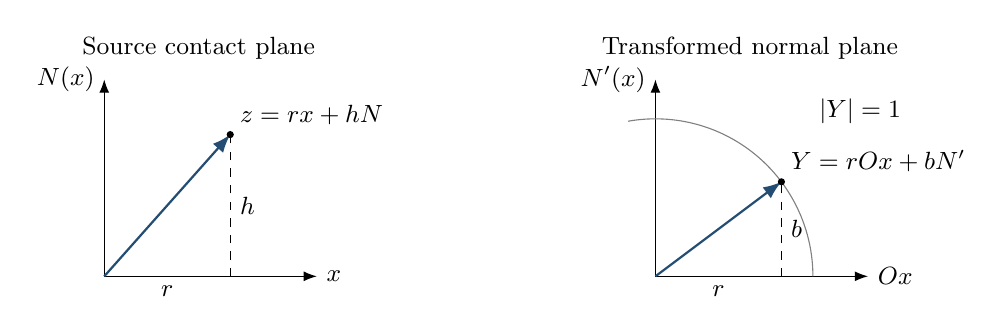
\begin{tikzpicture}[>=Latex,font=\small]
  \begin{scope}
    \node at (1.2,2.9) {Source contact plane};
    \draw[->] (0,0) -- (2.7,0) node[right] {$x$};
    \draw[->] (0,0) -- (0,2.5) node[left] {$N(x)$};
    \draw[dashed] (1.6,0) -- (1.6,1.8);
    \draw[thick,->,linkblue] (0,0) -- (1.6,1.8);
    \fill (1.6,1.8) circle (1.3pt);
    \node[above right] at (1.6,1.8) {$z=rx+hN$};
    \node[below] at (0.8,0) {$r$};
    \node[right] at (1.6,0.9) {$h$};
  \end{scope}
  \begin{scope}[xshift=7cm]
    \node at (1.2,2.9) {Transformed normal plane};
    \draw[->] (0,0) -- (2.7,0) node[right] {$Ox$};
    \draw[->] (0,0) -- (0,2.5) node[left] {$N'(x)$};
    \draw[gray] (2,0) arc[start angle=0,end angle=100,radius=2];
    \draw[dashed] (1.6,0) -- (1.6,1.2);
    \draw[thick,->,linkblue] (0,0) -- (1.6,1.2);
    \fill (1.6,1.2) circle (1.3pt);
    \node[above right] at (1.6,1.2) {$Y=rOx+bN'$};
    \node[below] at (0.8,0) {$r$};
    \node[right] at (1.6,0.6) {$b$};
    \node at (2.6,2.1) {$|Y|=1$};
  \end{scope}
\end{tikzpicture}
\caption{The two decompositions at a fixed closest-point contact, shown
schematically with positive normal coefficients. Lorentz invariance
makes the coefficient $r=\sqrt{1-b^2}$ the same in both planes.
The source vector $z$ need not be unit length. On a fixed level, $b$
is constant while $h=h_{v,b}(x)$ can vary. The isometry $O$ and normal
$N'$ depend on the source point; the picture does not represent a
single ambient rotation.}
\label{fig:family-normal-planes}
\end{figure}

Differentiating $N'$ and then $Y_{v,b}$, with $v,b$ fixed, gives
\[
 dN'=D^{-1}\bigl(B\,dN+S\,dg\,N'\bigr)=D^{-1}O\,dN,
\]
and consequently
\begin{equation}\label{eq:family-jacobian}
 \begin{split}
 dY_{v,b}
 &=rO\,dx+(b+rSf)D^{-1}O\,dN
   =O(rI-h_{v,b}A),\\
 J_mY_{v,b}&=\bigl|\det(rI-h_{v,b}A)\bigr|.
 \end{split}
\end{equation}
Here $J_m$ is the metric $m$-dimensional Jacobian; the isometry $O$
accounts for the entire ambient change in the differential.

\subsection{Every level has the required perimeter bound}

Define
\[
 E_{v,b}=\{y\in S^{m+1}:\psi_v(y)<b\},\qquad
 \Lambda_{v,b}=\{y\in S^{m+1}:\psi_v(y)=b\}.
\]
For finite boosts and interior levels, also define the closed source set
\[
 T_{v,b}=\{x\in\Sigma:rI-h_{v,b}(x)A(x)\ge0\}.
\]

\begin{lemma}[The restricted area bound]\label{lem:family-all-levels}
Every $E_{v,b}$, for $(v,b)\in Q$, has finite perimeter.
For $|v|<1$, $|b|<1$ and every open set $U\subset S^{m+1}$,
\begin{equation}\label{eq:family-restricted-perimeter}
 \begin{split}
 \operatorname{Per}(E_{v,b};U)
 &\le\mathcal H^m(\Lambda_{v,b}\cap U)\\
 &\le\int_{T_{v,b}\cap Y_{v,b}^{-1}(U)}
       \det(rI-h_{v,b}A)\,d\mu,
 \end{split}
\end{equation}
and on $T_{v,b}$,
\begin{equation}\label{eq:family-restricted-density}
 0\le\det(rI-h_{v,b}A)\le r^m\le1.
\end{equation}
Thus these estimates hold at every level, without an exceptional set
of values of $b$.
\end{lemma}

\begin{proof}
Take $y\in\Lambda_{v,b}$ and transform $(y,b)$ to $(z,h)$ by
\eqref{eq:family-boost}.  Lemma~\ref{lem:family-cone-contact} supplies
a closest point $r_zx$.  Lorentz invariance gives
$r_z^2=|z|^2-h^2=1-b^2$, so $r_z=r$.
The inverse formulas then show that $h=h_{v,b}(x)$,
$y=Y_{v,b}(x)$, and $x\in T_{v,b}$.  Therefore
\begin{equation}\label{eq:family-level-cover}
 \Lambda_{v,b}\subset Y_{v,b}(T_{v,b}).
\end{equation}
The nonnegative eigenvalues of $rI-h_{v,b}A$ have sum $mr$, because
$\tr A=0$.  Their arithmetic--geometric mean inequality proves
\eqref{eq:family-restricted-density}. The area formula
\cite[\S3.2.3]{Federer1969}\ \cite[\S3, pp.~299--300]{Federer1978},
with multiplicities counted in its source
integral, now yields the second inequality in
\eqref{eq:family-restricted-perimeter}.
The condition defining $T_{v,b}$ is only necessary for a closest-point
contact.  Additional points in this source set, and multiple preimages
of a level point, increase the upper bound and cause no difficulty.

In particular $\mathcal H^m(\Lambda_{v,b})<\infty$.
Since $E_{v,b}$ is open, its essential boundary is contained in its
topological boundary, which is contained in $\Lambda_{v,b}$.
The finite-essential-boundary criterion
\cite[\S4, p.~302]{Federer1978}, applied in coordinate charts, gives
finite perimeter. The intrinsic reduced-boundary representation
\cite[\S2.2]{BDFSphere} then gives
\[
 \operatorname{Per}(E_{v,b};U)
 =\mathcal H^m(\partial^*E_{v,b}\cap U)
 \le\mathcal H^m(\Lambda_{v,b}\cap U).
\]
This proves the first inequality with constant one.

For $|v|<1$ the endpoint sublevels are empty and full, respectively.
For $|v|=1$, formula~\eqref{eq:family-boundary-graph} makes them round
caps, whose boundary masses are $\sigma_m(1-b^2)^{m/2}$, with zero
mass at $b=\pm1$.  These cases also have finite perimeter.
\end{proof}

All of the levels $\Lambda_{v,b}$ have zero $(m+1)$-dimensional volume:
this follows from their finite $m$-dimensional measure in the interior;
on the boost boundary they are round spheres or singletons; and at
finite-boost endpoints they are empty.
If $(v_j,b_j)\to(v,b)$, Lemma~\ref{lem:family-graph} gives uniform
convergence of $\psi_{v_j}-b_j$ to $\psi_v-b$.  Indicators of the
sublevels consequently converge pointwise off $\Lambda_{v,b}$.
Dominated convergence proves
\begin{equation}\label{eq:family-filling-continuity}
 \Vol_{m+1}(E_{v_j,b_j}\mathbin\triangle E_{v,b})\longrightarrow0.
\end{equation}
Thus
\[
 \widehat\Phi(v,b)=\partial[E_{v,b}]
\]
is flat continuous on $Q$, since the flat distance between two of these
cycles is at most the volume of the symmetric difference of their
fillings.  Its mass equals the perimeter of the filling, so
\eqref{eq:family-mass-bounds} follows from
Lemma~\ref{lem:family-all-levels}.

\subsection{Infinite boosts and no concentration of mass}

We have obtained a flat-continuous family with the required total mass
bound. To apply the min--max theorem, we must also control its mass in
small balls uniformly over parameters, including boosts tending to
infinity. The restricted Jacobian estimate lets us do this on the one
fixed compact source \(\Sigma\).

\begin{lemma}[No concentration]\label{lem:family-no-concentration}
The family $\widehat\Phi$ satisfies
\begin{equation}\label{eq:family-no-concentration}
 \lim_{\rho\downarrow0}\;
 \sup_{(v,b)\in Q}\sup_{y\in S^{m+1}}
 \|\widehat\Phi(v,b)\|(B_\rho(y))=0.
\end{equation}
\end{lemma}

\begin{proof}
We prove the sequential form of the assertion.  Consider
$u_j=(v_j,b_j)\to(v_*,b_*)$, $y_j\to y_*$, and $\rho_j\downarrow0$.
The case $|b_*|=1$ follows directly from
\eqref{eq:family-mass-bounds}.  Parameters on $|v|=1$ are harmless as
well: an $m$-sphere of Euclidean radius $r$ in any affine
$(m+1)$-plane has at most $c_m\rho^m$ area in a ball of radius $\rho$,
uniformly in $r$ and the plane.  For $r\le2\rho$ use its total area;
for $r>2\rho$ the intersection lies in a spherical cap with angular
radius at most $\arcsin(\rho/r)$, and the same bound follows by the
cap area formula.  Spherical balls in the ambient unit sphere lie in
Euclidean balls of the same radius.  We may therefore pass to a
subsequence with $|v_j|<1$ and $|b_*|<1$.

Put $Y_j=Y_{v_j,b_j}$ and $T_j=T_{v_j,b_j}$.
The local perimeter bound reduces the desired assertion to
\begin{equation}\label{eq:family-concentration-integrands}
 \int_\Sigma I_j\,d\mu\longrightarrow0,
 \qquad
 I_j=\mathbf1_{T_j}\,
      \mathbf1_{Y_j^{-1}(B_{\rho_j}(y_j))}\,J_mY_j.
\end{equation}
The restricted bound gives $0\le I_j\le1$ on the fixed compact source.

If $|v_*|<1$, the maps $Y_j$ converge smoothly on $\Sigma$ to
$Y_*=Y_{v_*,b_*}$.  Away from the fiber $Y_*^{-1}(y_*)$, the ball
indicator in \eqref{eq:family-concentration-integrands} eventually
vanishes.  The area formula applied to the fiber gives
\[
 \int_{Y_*^{-1}(y_*)}J_mY_*\,d\mu=0,
\]
because a singleton has zero $\mathcal H^m$ measure.
Thus $J_mY_*=0$ almost everywhere on that fiber, and smooth
convergence gives $I_j\to0$ there almost everywhere as well.
Dominated convergence completes this case.

It remains to consider $v_*=a$ with $|a|=1$.
Write $a_j=v_j/|v_j|$, $t_j=S_j/C_j=|v_j|$, and
$f_j=\langle a_j,x\rangle$, $g_j=\langle a_j,N\rangle$.
The cancellation identity
\begin{equation}\label{eq:family-cancelled-map}
 Bx+SfN'=x+f\,\frac{SN-(C-1)a}{D}
\end{equation}
gives
\[
 Y_j=r_j\left[x+
 f_j\frac{t_jN-(1-C_j^{-1})a_j}{1-t_jg_j}\right]+b_jN'_j.
\]
On compact subsets of $\Sigma\setminus Z_a$, where
$Z_a=\{x:N(x)=a\}$, the denominators stay uniformly positive.
Also
\[
 N'_j=
 \frac{C_j^{-1}N+(1-C_j^{-1})g_ja_j-t_ja_j}{1-t_jg_j}
 \longrightarrow-a.
\]
The maps and all their source derivatives therefore converge locally
to
\begin{equation}\label{eq:family-infinite-map}
 Y_\infty(x)=r_*\left[x+
       \frac{\langle a,x\rangle}{1-\langle a,N\rangle}(N-a)
                 \right]-b_*a,
 \qquad r_*=\sqrt{1-b_*^2}.
\end{equation}
This computation allows the directions $a_j$ to vary.

The exceptional normal fiber $Z_a$ is source-null.
Indeed $Z_a\subset\{x:\langle a,x\rangle=0\}$, whereas
$\langle a,x\rangle$ is a nontrivial analytic function by
Lemma~\ref{lem:fullness}.  Its zero set has zero $m$-dimensional
measure.  No rank assumption on the Gauss map is involved.

The point fiber $F=Y_\infty^{-1}(y_*)$, defined off $Z_a$, may instead
have positive source measure.  On a countable cover by relatively
compact coordinate patches in $\Sigma\setminus Z_a$, the area formula
gives
\[
 \int_{F\cap K}J_mY_\infty\,d\mu=0
\]
for each such patch $K$.  Hence $J_mY_\infty=0$ almost everywhere on
$F$.  Off $F\cup Z_a$ the shrinking-ball indicator is eventually
zero; on $F$, local smooth convergence gives $J_mY_j\to0$ almost
everywhere.  We conclude that $I_j\to0$ almost everywhere on
$\Sigma$, and $0\le I_j\le1$ again permits dominated convergence.
In particular, convergence of the indicators $\mathbf1_{T_j}$ is
unnecessary.  Only the restricted Jacobians are bounded; no bound for
the unrestricted $J_mY_j$ near $Z_a$ has been used.

Finally, if \eqref{eq:family-no-concentration} failed, compactness of
$Q$ and $S^{m+1}$ would supply sequences of the above form whose ball
masses stay bounded below by a positive constant.  The sequential
result excludes them.
\end{proof}

\subsection{The projective parameter space}

On $|v|=1$, formula~\eqref{eq:family-boundary-graph} gives
\[
 E_{v,b}=\{\langle v,y\rangle>-b\},\qquad
 E_{-v,-b}=\{\langle v,y\rangle<-b\}.
\]
These fillings are complementary modulo their null common level.
On the top and bottom faces they are full and empty, respectively.
Together with the volume continuity in
\eqref{eq:family-filling-continuity}, these facts verify every
hypothesis of Lemma~\ref{lem:minmax-projective}. Therefore
$\widehat\Phi(u)=\partial[E_u]$ descends to a flat-continuous detecting
map $\Phi$ on $\mathbb {RP}^{p}$. Its image is unchanged by passage to
the quotient, so Lemma~\ref{lem:family-no-concentration} also gives no
concentration for $\Phi$.

At $(0,0)$, $\psi_0=\varphi$ on the sphere, and the level is
$\Sigma$, with sublevel $\Omega$.  Combining the upper mass bound,
Lemma~\ref{lem:family-no-concentration}, and
Lemma~\ref{lem:detection-gap} proves part~\textup{(i)} of
Proposition~\ref{prop:lorentz-family}, in particular
\begin{equation}\label{eq:family-gap}
 |\Sigma|\ge\gamma_m>\sigma_m.
\end{equation}

\subsection{Uniform area loss away from the center}

The family now detects the required cohomology class and has no
concentration. We next prove that all parameters away from the original
hypersurface lose a uniform amount of area. This isolates the maximum
that the extra negative direction will remove.

\begin{lemma}[A fixed source patch gives strict loss]
\label{lem:family-strict-loss}
For every neighborhood $U$ of $(0,0)$,
\eqref{eq:family-away-gap} holds.
\end{lemma}

\begin{proof}
Suppose otherwise.  There are $u_j=(v_j,b_j)\in Q\setminus U$ with
$\mathbf M(\widehat\Phi(u_j))\to|\Sigma|$.
The mass bound forces $b_j\to0$.
Parameters on the boost boundary have mass at most $\sigma_m$, which
is strictly smaller by \eqref{eq:family-gap}; discard those terms.
After taking a subsequence, $v_j\to v_*\ne0$.
Set $t_*=|v_*|\in(0,1]$ and $a=v_*/|v_*|$.
Discard finitely many terms so that $v_j\ne0$.
For each $j$, set $t_j=|v_j|$, $a_j=v_j/|v_j|$,
$C_j=(1-t_j^2)^{-1/2}$, $r_j=\sqrt{1-b_j^2}$,
$f_j=\langle a_j,x\rangle$, and $g_j=\langle a_j,N\rangle$.

The open set $\{A\ne0\}$ is nonempty.  The analytic function
$f=\langle a,x\rangle$ cannot vanish on that entire open set, by
fullness and connectedness.  Choose a compact source patch $K_0$ of
positive measure on which $|A|$ and $|f|$ are bounded below by
positive constants.  It is also disjoint from $\{N=a\}$, because
$N=a$ implies $f=0$.
On this fixed patch, the formula for $h_j=h_{v_j,b_j}$ becomes
\[
 h_j=\frac{b_j/C_j+t_jr_jf_j}{1-t_jg_j}
 \longrightarrow
 h_*:=\frac{t_*f}{1-t_*\langle a,N\rangle},
\]
uniformly.  Its limit is finite and nonzero on $K_0$, including when
$t_*=1$.

For a real symmetric matrix $M$, define its truncated determinant by
\[
 \mathcal D(M)=
 \begin{cases}
  \det M,&M\ge0,\\
  0,&M\not\ge0.
 \end{cases}
\]
This is continuous: every boundary point of the positive-semidefinite
cone is singular, so its determinant vanishes.
At every $x\in K_0$, the matrix $I-h_*(x)A(x)$ has trace $m$ and is
not the identity.  If it is positive semidefinite, strictness in the
arithmetic--geometric mean inequality gives determinant less than
one; if it is not, $\mathcal D$ is zero.
Compactness of $K_0$ and continuity therefore give $\delta>0$ with
\[
 \mathcal D(I-h_*A)\le1-2\delta\quad\hbox{on }K_0.
\]
For all large $j$ this yields
$\mathcal D(r_jI-h_jA)\le r_j^m-\delta$ on $K_0$.
On all of $\Sigma$, the restricted determinant is at most $r_j^m$.
Thus the area formula estimate gives
\[
 \mathbf M(\widehat\Phi(u_j))
 \le\int_\Sigma\mathcal D(r_jI-h_jA)\,d\mu
 \le r_j^m|\Sigma|-\delta\mu(K_0),
\]
contradicting convergence to $|\Sigma|$.
The proof supplies a uniform loss on a fixed portion of the source;
it makes no upper-semicontinuity assumption about area in the flat
topology.
\end{proof}

\subsection{The entire central level is a smooth boundary}

\begin{lemma}[The central tube]\label{lem:family-central-tube}
For all sufficiently small $(v,b)$, the entire level
$\Lambda_{v,b}$ is $Y_{v,b}(\Sigma)$, with $Y_{v,b}$ a smooth
embedding depending smoothly on the parameters.  Every level point
has a unique closest-point contact in the cone representation.
Moreover
\begin{equation}\label{eq:family-regular-level}
 \nabla_{S^{m+1}}\psi_v=N'-bY_{v,b},\qquad
 |\nabla_{S^{m+1}}\psi_v|=r>0
 \quad\hbox{on }\Lambda_{v,b}.
\end{equation}
Thus $\Lambda_{v,b}=\partial E_{v,b}=\partial^*E_{v,b}$ and its
boundary cycle has multiplicity one.
\end{lemma}

\begin{proof}
Use a tubular neighborhood of the smooth cone on a compact annulus
containing $\{sx:x\in\Sigma,\ 1/2\le s\le3/2\}$, constructed inside
a slightly larger annulus.  Compact embeddedness supplies a uniform
$\epsilon>0$ so that, for these central radii and $|h|<\epsilon$,
the point $sx+hN(x)$ has unique closest cone point $sx$, and signed
distance $h$.  This is a tube for the whole cone: after shrinking
$\epsilon$, points at radii outside the larger annulus cannot be
closest, and uniqueness within that annulus follows from its tubular
neighborhood.

For any actual level point $y\in\Lambda_{v,b}$, the boost gives
\[
 |h|=|Cb+S\langle a,y\rangle|\le C|b|+S\longrightarrow0
 \quad\hbox{as }(v,b)\to(0,0).
\]
Every closest cone point has radius $r=\sqrt{1-b^2}\to1$.
Thus all actual contacts lie in this one fixed tube, so each is
unique.  Conversely, for every source point $x$, the inverse formula
gives
\[
 |h_{v,b}(x)|\le\frac{|b|+Sr}{C-S}\longrightarrow0
\]
uniformly on $\Sigma$.
Consequently $z=rx+h_{v,b}(x)N(x)$ lies in the same tube and really
has signed distance $h_{v,b}(x)$.  Its transformed point
$Y_{v,b}(x)$ is therefore an actual level point.
This proves equality with the entire level and uniqueness of its
source representation, not merely existence of one nearby component.

For these parameters the matrix $rI-h_{v,b}A$ is uniformly positive
definite, so \eqref{eq:family-jacobian} gives an immersion.
Uniqueness of the contact and invertibility of the boost give
injectivity; compactness then gives an embedding.
All the formulas are smooth in $(v,b,x)$ near the center.

In the tube $d\varphi=N\cdot dz$.  Differentiating the graph relation
at one of the level points yields
\[
 0=dh-N\cdot dz
  =D\bigl(db-N'\cdot dy\bigr).
\]
The derivative with respect to $b$ is $D>0$, so the graph is smooth
near that point and its Euclidean gradient is $N'$.
Projecting onto the tangent space of the unit sphere and using
\eqref{eq:family-orthogonal-decomposition} proves
\eqref{eq:family-regular-level}.
Each level point therefore has a neighborhood in which $E_{v,b}$ is
one side of a regular smooth hypersurface.  This proves the claimed
topological and reduced boundary identities, with multiplicity one.
\end{proof}

\subsection{The extra index direction removes the maximum}

Expand the central embedding in the Euclidean parameter
$u=(v,b)\in\mathbb R^p$:
\begin{equation}\label{eq:family-first-variation}
 Y_{v,b}(x)=x+(b+\langle v,x\rangle)N(x)+O(|u|^2).
\end{equation}
The error is smooth and uniform with its source derivatives.
The functions in \eqref{eq:family-normal-variations} are independent:
integrating a relation $t+\langle d,x\rangle=0$ gives $t=0$, and
fullness then gives $d=0$.
To evaluate their second variation, use $L=\Delta+m+P$, $P=|A|^2$,
and write $w=t+f$, $f=\langle d,x\rangle$.
Since $\Delta f=-mf$ and $\int_\Sigma f\,d\mu=0$,
\begin{equation}\label{eq:family-positive-form}
 \int_\Sigma wLw\,d\mu
   =m|\Sigma|t^2+\int_\Sigma P(t+f)^2\,d\mu>0
 \qquad\text{if }(d,t)\ne0.
\end{equation}
For $t\ne0$ the first term suffices.  For $t=0$, $d\ne0$, the
nontrivial analytic function $f$ cannot vanish throughout the nonempty
open set where $P>0$.
The minimal second-variation formula is
$\delta^2\Area(w,w)=-\int_\Sigma wLw\,d\mu$.
Lemma~\ref{lem:family-central-tube} ensures that it computes the mass
of the actual boundary family, proving part~\textup{(iii)} of the
proposition.

Assume now that $\ind(\Sigma)>p$.  Let
\[
 W=\{t+\langle d,x\rangle:t\in\mathbb R,\ d\in\mathbb R^{m+2}\},
 \qquad
 \mathcal B(\phi,\chi)=\int_\Sigma\phi L\chi\,d\mu.
\]
Choose a finite-dimensional subspace spanned by $L$-eigenfunctions
with positive eigenvalues, of dimension greater than $p$.
The $p$ linear conditions
$\mathcal B(\eta,w)=0$ for $w\in W$ admit a nonzero smooth solution
$\eta$ in that subspace.  Then $\mathcal B(\eta,\eta)>0$, and
\eqref{eq:family-positive-form} implies that $\mathcal B$ is positive
definite on $W\oplus\mathbb R\eta$.

Extend $\eta N$ to a smooth ambient vector field on $S^{m+1}$, and
let $F_s$ be its flow.  For small $u,s$, set
\[
 E(u,s)=F_s(E_u),\qquad
 \mathcal A(u,s)=\operatorname{Per}(E(u,s)),
 \qquad E_u=E_{v,b}.
\]
Lemma~\ref{lem:family-central-tube} makes $\mathcal A$ smooth in a neighborhood
of $(0,0)$.  Its first derivative there vanishes by minimality, and
its Hessian is negative definite, by the preceding positive-form
calculation.  Taylor's theorem therefore gives constants $c>0$ and
$\delta>0$ such that
\begin{equation}\label{eq:family-morse-estimate}
 \mathcal A(u,s)\le|\Sigma|-c(|u|^2+s^2)
 \qquad\text{when }|u|^2+s^2\le\delta^2.
\end{equation}
Shrink $\delta$ so that this ball lies inside the central smooth
parameter region.

Choose a smooth nonnegative function $\beta(u)$ supported in
$|u|<\delta/2$ and equal to one near $u=0$.
For sufficiently small $\varepsilon>0$, replace $E_u$ on that region
by $E(u,\varepsilon\beta(u))$ and leave it unchanged elsewhere.
The compact graph
\[
 \{(u,\varepsilon\beta(u)):|u|\le\delta/2\}
\]
misses $(0,0)$.  It is contained in the ball on which
\eqref{eq:family-morse-estimate} holds, so its area maximum is
strictly below $|\Sigma|$.
On the complement of $|u|<\delta/2$, the same strict upper bound,
possibly with a different positive gap, follows from
Lemma~\ref{lem:family-strict-loss}.
The boundaries of the modified domains consequently define a map
$\widetilde\Phi$ satisfying \eqref{eq:family-strict-deformation}.

Replacing $\varepsilon$ by $t\varepsilon$, $0\le t\le1$, gives a
flat homotopy, fixed outside the chosen interior neighborhood of $Q$.
It descends through the quotient and preserves the detecting class.
On the modified region, the boundaries belong to a compact smooth
family of embeddings of $\Sigma$, and hence have no concentration
of mass.  For completeness, a finite cover by coordinate graph
patches, with uniform metric and first-derivative bounds over the
compact parameter set, bounds their masses in radius-$\rho$ balls
by a constant times $\rho^m$.  Outside that region the original
no-concentration estimate applies unchanged.
This proves part~\textup{(iv)}.  Part~\textup{(ii)} is
Lemma~\ref{lem:family-strict-loss}, so the proof of
Proposition~\ref{prop:lorentz-family} is complete.

\section{Low-density cones and attainment}\label{sec:cones}

We now obtain the compactness needed to minimize among counterexamples.
The regularity argument has two induction parameters: the hypersurface
dimension $m$ in Theorem~\ref{thm:volume}, and the dimension of a Euclidean
cone.  Keeping them separate is essential.  The theorem in dimensions
less than $m$ will classify cones of dimension at most $m$, and these
classifications will give a smooth link for a cone of dimension $m+1$.

For a varifold $V$, its weight measure is
$\|V\|$ and its total mass, when finite, is $\mathbf M(V)$.
For a smooth embedded submanifold $S$, write $\mathbf v(S)$ for its
associated varifold with multiplicity one.
For an integral $k$-varifold in Euclidean space, $[V]$ denotes the
locally rectifiable flat chain with coefficients in $\mathbb Z_2$
obtained by reducing its integer multiplicity modulo two.  We call
$V$ \emph{cyclic modulo two} if $\partial[V]=0$ locally in the ambient
open set.  This convention applies to noncompact cones and their
translates, using locally flat chains as in
\cite[\S2.1 and Appendix]{White2009}.

\subsection{Coning, density, and the radial factor}

\begin{lemma}[The cone operation]\label{lem:cone-operation}
Let $d\geq1$ and let $V$ be a stationary integral $d$-varifold in the
unit sphere $S^{d+1}$.  Its Euclidean cone $\mathcal C(V)$ is a
stationary integral $(d+1)$-varifold in $\mathbb R^{d+2}$, and
\begin{equation}\label{eq:cones-mass}
 \|\mathcal C(V)\|(B_R(0))
   =\frac{R^{d+1}}{d+1}\mathbf M(V),
 \qquad
 \Theta(\mathcal C(V),0)=\frac{\mathbf M(V)}{\sigma_d}.
\end{equation}
If $V$ is a finite sum of smooth closed embedded minimal
hypersurfaces with positive integer multiplicities, then
$\mathcal C(V)$ is cyclic modulo two.
\end{lemma}

\begin{proof}
At a spherical point $x$ with tangent plane $P\subset x^\perp$, assign
to $rx$ the plane $\mathbb Rx\oplus P$ and the measure
$r^d\,dr\,dV(x,P)$.  This defines the cone and gives
\eqref{eq:cones-mass}.  The polar map is a diffeomorphism away from
the origin; rectifiability and integer multiplicity there follow
from the area formula.  The origin has zero mass.

For stationarity, first take a smooth ambient field $X$ supported
away from the origin and write
$X(rx)=f(r,x)x+Y_r(x)$, where $Y_r(x)\perp x$.
The trace of its derivative on the cone plane is
\[
 \operatorname{div}_{\mathbb Rx\oplus P}X(rx)
 =\partial_r f(r,x)+\frac{d}{r}f(r,x)
       +\frac1r\operatorname{div}^{S}_{P}Y_r(x).
\]
After multiplication by $r^d$ and integration, the first two terms
integrate to the endpoint values of $r^df$, and the last term
vanishes by spherical stationarity for each $r$.  Thus the cone is
stationary off the origin.  For a general compactly supported $X$,
insert a radial cutoff that is zero on $B_\varepsilon$ and one
outside $B_{2\varepsilon}$, with derivative bounded by
$c/\varepsilon$.  Formula~\eqref{eq:cones-mass} bounds the omitted
first-variation terms by
$c_X(\varepsilon^{d+1}+\varepsilon^d)$, which tends to zero.

For the last assertion, $[\mathcal C(V)]$ has zero boundary on
every annulus: an odd component multiplicity gives a smooth
mod-two product cylinder, and an even multiplicity gives zero.
Truncate this chain inside radius $\varepsilon$.  Its difference
from the full chain has mass at most
$\mathbf M(V)\varepsilon^{d+1}/(d+1)$, whereas its inner boundary
has mass at most $\mathbf M(V)\varepsilon^d$.
The truncated chains therefore converge locally flat to
$[\mathcal C(V)]$ and their boundaries converge locally flat to zero.
Continuity of the boundary operator proves
$\partial[\mathcal C(V)]=0$ also at the vertex.
\end{proof}

We use the stationary monotonicity formula, tangent-cone existence,
and integral-varifold closure of Allard
\cite[\S5 and Theorem~6.4]{Allard1972}; see also the formulations in
\cite[Chapter~4, \S3]{SimonGMT} and
\cite[Theorem~3.2]{White2009}.
In particular, on a fixed open set, locally bounded mass and locally
bounded first variation give a subsequence with an integral-varifold
limit.  For the stationary sequences below the first variation is
identically zero.  White's convergence theorem then gives the
additional implication
\begin{equation}\label{eq:cones-white}
 V_i\longrightarrow V,\quad \delta V_i=0,\quad
 \partial[V_i]=0
 \quad\Longrightarrow\quad \partial[V]=0,
\end{equation}
provided the masses are locally bounded.  Indeed, Allard gives
integrality of $V$; the first variations satisfy White's local bound
with bound zero; and the boundary chains converge to zero.
These are precisely the hypotheses of
\cite[Definition~3.1 and Theorem~3.3]{White2009}.
The same statement applies after any translations and dilations,
and hence to the blow-ups used below.

\begin{lemma}[Density at every support point]\label{lem:cones-density}
Let $V$ be a stationary integral $k$-varifold in an open set
$U\subset\mathbb R^n$.  At every $z\in\spt\|V\|$,
$\Theta(V,z)\geq1$.  If $V=\mathcal C$ is a cone in all of
$\mathbb R^n$, then
\begin{equation}\label{eq:cones-density-comparison}
 1\leq\Theta(\mathcal C,z)\leq\Theta(\mathcal C,0)
 \qquad (z\in\spt\|\mathcal C\|).
\end{equation}
Every tangent cone at such a point is nonzero and has density
$\Theta(\mathcal C,z)$ at its vertex.
\end{lemma}

\begin{proof}
Integrality gives density at least one at $\|V\|$-almost every point.
Every neighborhood of $z$ has positive mass, so choose such points
$x_i\to z$.  If $\overline{B_r(z)}\subset U$ and
$d_i=|x_i-z|<r$, monotonicity at $x_i$ and ball inclusion give
\[
 \|V\|(B_r(z))\geq\|V\|(B_{r-d_i}(x_i))
       \geq\omega_k(r-d_i)^k.
\]
Let $i\to\infty$, then $r\downarrow0$.  This proves the asserted
lower bound also at support points that are exceptional for
rectifiability.

For a cone, its homogeneous mass measure gives
$\|\mathcal C\|(B_R(0))=\omega_k\Theta(\mathcal C,0)R^k$.
For $R>|z|$, the inclusions
\[
 B_{R-|z|}(0)\subset B_R(z)\subset B_{R+|z|}(0)
\]
identify the limit of the mass ratios centered at $z$ as
$R\to\infty$ with $\Theta(\mathcal C,0)$.
Monotonicity proves the upper bound in
\eqref{eq:cones-density-comparison}.  Tangent-cone existence and
the monotonicity formula give the stated tangent density, which is
positive by the first part.
\end{proof}

\begin{lemma}[Splitting the radial line]\label{lem:cones-splitting}
Let $k\geq2$ and let $\mathcal C$ be a stationary integral
$k$-dimensional cone in $\mathbb R^{k+1}$.
For $0\ne z\in\spt\|\mathcal C\|$, every tangent cone $T$ at $z$
has the form
\[
 T=\mathbf v(\mathbb Re)\times W,\qquad e=z/|z|,
\]
where $W$ is a nonzero stationary integral $(k-1)$-dimensional
cone in $e^\perp\cong\mathbb R^k$ and
\begin{equation}\label{eq:cones-factor-density}
 \Theta(W,0)=\Theta(T,0)=\Theta(\mathcal C,z).
\end{equation}
If $\mathcal C$ is cyclic modulo two, so are $T$ and $W$.
\end{lemma}

\begin{proof}
Write $T_i=(\eta_{z,\rho_i})_\#\mathcal C\to T$, where
$\eta_{z,\rho_i}(y)=(y-z)/\rho_i$ and $\rho_i\downarrow0$.
For fixed $b\in\mathbb R$, dilation invariance of $\mathcal C$
by the positive factors $1+b\rho_i$ implies invariance of $T_i$
under
\[
 y\longmapsto(1+b\rho_i)y+bz.
\]
Passing to the limit shows that $T$ is invariant under translation
by $bz$.  Its weight consequently disintegrates as
$\|T\|=\mathcal L^1\otimes\nu$ on
$\mathbb Re\oplus e^\perp$.

We check that this is an integral varifold product.
At almost every rectifiable point of $T$, a measure blow-up is an
integer multiple of the measure on its approximate tangent plane.
These blow-ups retain invariance under translations in the
$e$-direction, so that plane contains $e$.
The tangential Jacobian of the coordinate
$\pi(te+w)=t$ is therefore one almost everywhere.
Rectifiable coarea gives, for almost every $t$, a
$(k-1)$-rectifiable slice with the original integer multiplicities;
its tangent plane is the intersection of the tangent plane of $T$
with $e^\perp$.  Product disintegration identifies the weight of
this slice, after translation to $e^\perp$, with $\nu$.
Thus $\nu$ defines an integral varifold $W$ and the tangent-plane
identification gives $T=\mathbf v(\mathbb Re)\times W$ as varifolds.
Here we use rectifiable coarea
\cite[\S3, p.~300]{Federer1978}.

For a compactly supported field $Y$ on $e^\perp$ and a compactly
supported smooth function $\chi$ on $\mathbb R$ with
$\int\chi\ne0$, test stationarity of $T$ with
$X(te+w)=\chi(t)Y(w)$.  Since $Y$ is perpendicular to $e$,
\[
 0=\delta T(X)=\left(\int_{\mathbb R}\chi(t)\,dt\right)\delta W(Y).
\]
Hence $W$ is stationary.  Dilation invariance of the tangent cone
$T$ and the product formula imply dilation invariance of $W$.
Writing $\theta=\Theta(W,0)$, integration over a ball gives
\[
 \|T\|(B_1)
 =\theta\omega_{k-1}
       \int_{-1}^1(1-t^2)^{(k-1)/2}\,dt
 =\theta\omega_k.
\]
This proves \eqref{eq:cones-factor-density};
Lemma~\ref{lem:cones-density} makes $W$ nonzero.

If $\partial[\mathcal C]=0$, every $T_i$ is cyclic, and
\eqref{eq:cones-white} implies $\partial[T]=0$.
The mod-two slicing identity for the boundary
\cite[\S3, equation~(1) and Proposition~3.1]{White1999} gives
\[
 \partial\langle[T],\pi,t\rangle
       =\langle\partial[T],\pi,t\rangle=0
 \quad\text{for almost every }t,
\]
where signs disappear modulo two. For the locally flat chain, apply
the identity on a countable exhaustion by relatively compact regions;
restriction compatibility gives one full-measure set of levels where
it holds locally everywhere. Choose one such level where the preceding
rectifiable slice description also holds. The slice there is the
translate of $[W]$ to $te+e^\perp$,
because $T$ is the product just established.  Translation back
proves $\partial[W]=0$.  No assertion about whether zero is a good
slicing level is needed.
\end{proof}

For clarity, we also record the precise regularity consequence
used in the dimension reduction.

\begin{lemma}[A multiplicity-one planar tangent]\label{lem:cones-allard}
Let $V$ be a stationary integral $k$-varifold, $k\geq2$, in an open
subset of Euclidean space.  If one tangent cone at $z$ is a
multiplicity-one plane, then in a neighborhood of $z$, $V$ is a
smooth embedded minimal submanifold with multiplicity one.
\end{lemma}

\begin{proof}
Apply Allard's interior regularity theorem
\cite[\S8]{Allard1972}, in the formulation of
\cite[Chapter~5, hypotheses~(5.1) and Theorem~5.2]{SimonGMT},
on a sufficiently small rescaled ball from
the sequence giving that tangent.  Its hypotheses hold as follows.
Integrality supplies the almost-everywhere density lower bound one.
Stationarity supplies zero generalized mean curvature and zero
first variation, hence the required mean-curvature bound for any
exponent greater than $k$.  Convergence to the multiplicity-one
plane supplies normalized mass arbitrarily close to $\omega_k$
and arbitrarily small height and tangent-plane excess on a fixed
smaller ball.  The center remains in the support.  Allard's theorem
therefore gives a single $C^{1,\alpha}$ graph near the center.
On that connected graph the stationary integral multiplicity is
constant; its tangent multiplicity is one, so the constant is one.
The higher-regularity conclusion of
\cite[Chapter~5, Theorem~6.1]{SimonGMT}, applied with the smoothly
prescribed mean curvature identically zero, makes the graph smooth;
that statement permits arbitrary codimension. This theorem has
no stability hypothesis and no upper bound on $k$.
\end{proof}

\Needspace{17\baselineskip}
\subsection{The cone induction}

\begin{proposition}[Low-density cones]\label{prop:low-density-cones}
Fix $m\geq2$ and assume Theorem~\ref{thm:volume} in dimensions
$2,\ldots,m-1$, with an empty assumption when $m=2$.
Let $\mathcal C$ be a nonzero stationary integral
$k$-dimensional cone in $\mathbb R^{k+1}$ such that
\begin{equation}\label{eq:cones-threshold}
 \Theta(\mathcal C,0)<\vartheta_m.
\end{equation}
When $m=2$ or $m=3$, also assume that $\mathcal C$ is cyclic
modulo two.  Then:
\begin{enumerate}[label=\textup{(\roman*)}]
 \item if $1\leq k\leq m$, $\mathcal C$ is a
 multiplicity-one hyperplane;
 \item if $k=m+1$, $\mathcal C$ is smooth embedded with
 multiplicity one away from its vertex.  Its link in $S^{m+1}$
 is a smooth closed connected embedded minimal hypersurface.
\end{enumerate}
\end{proposition}

\begin{proof}
Hold $m$ fixed throughout.  We prove (i) by induction in $k$ and
then obtain (ii) from the final induction step.

An integral one-dimensional cone is a finite union of rays with
positive integer weights: radial slicing of its conical
rectifiable measure gives a zero-dimensional integral measure on
the unit circle, and local finiteness makes its total weight finite.
Write the distinct unit ray directions as $u_j$, their weights
as $q_j$, and $N=\sum_jq_j$.  Stationarity at the origin says
\[
 \sum_jq_ju_j=0,\qquad \Theta(\mathcal C,0)=N/2.
\]
If $m\geq4$, Lemma~\ref{lem:clifford-ratios} gives
$\vartheta_m\leq3/2$, so the strict bound
\eqref{eq:cones-threshold} gives $N<3$.
Nonzero stationarity excludes $N=1$, leaving two opposite rays of
weight one.  If $m=2$ or $3$, the same lemma gives
$\vartheta_m<2$, hence $N<4$; cyclicity says that the boundary
coefficient $N$ at the origin is even.  Again $N=2$ and balance
gives a multiplicity-one line.  This proves the base case in both
branches.

Suppose next that $2\leq k\leq m+1$ and that (i) has been proved
in dimension $k-1$.  At any nonzero support point $z$,
Lemma~\ref{lem:cones-splitting} expresses a tangent as
$\mathbf v(\mathbb R)\times W$.  Its factor is nonzero, stationary and
integral, is cyclic when required, and has density at most
$\Theta(\mathcal C,0)<\vartheta_m$ by
Lemma~\ref{lem:cones-density}.  The induction hypothesis makes
$W$ a multiplicity-one plane.  Thus this tangent of $\mathcal C$
is a multiplicity-one plane, and
Lemma~\ref{lem:cones-allard} proves smooth embedded
multiplicity-one structure near $z$.

It follows that $\Lambda=\spt\|\mathcal C\|\cap S^k$ is a smooth
closed embedded $(k-1)$-manifold.  The radial direction lies in
the cone tangent plane and is normal to the sphere, so this
intersection is transverse.  Polar coarea gives
$\mathcal C=\mathcal C(\mathbf v(\Lambda))$ with multiplicity one.
Reversing the angular first-variation calculation in
Lemma~\ref{lem:cone-operation} shows that $\Lambda$ is minimal
in $S^k$.

Each connected component $\Lambda_j$ is compact and minimal,
and its cone is stationary.  Lemma~\ref{lem:cones-density}
applied to that cone, together with \eqref{eq:cones-mass}, yields
\begin{equation}\label{eq:cones-component}
 \frac{\Vol(\Lambda_j)}{\sigma_{k-1}}\geq1.
\end{equation}
Since the total cone density is less than $\vartheta_m<2$,
there is only one component.

If $k=2$, a closed connected embedded minimal curve in $S^2$ is a
great circle by the geodesic equation, so its cone is a plane.
If $3\leq k\leq m$ and $\Lambda$ were not totally geodesic, the
outer induction in dimension $k-1$ would give
\[
 \Theta(\mathcal C,0)
   =\frac{\Vol(\Lambda)}{\sigma_{k-1}}
   \geq\vartheta_{k-1}\geq\vartheta_m,
\]
contrary to \eqref{eq:cones-threshold}.  Thus $\Lambda$ is a
great sphere and $\mathcal C$ a multiplicity-one plane, completing
(i).  For $k=m+1$, the already proved plane assertion in dimension
$m$ gives exactly the smoothness and connectedness asserted in
(ii).  We do not apply the dimension-$m$ volume statement to this
last link.
\end{proof}

\begin{corollary}[Spherical stationary output]\label{cor:cones-spherical-output}
Under the outer induction hypothesis of
Proposition~\ref{prop:low-density-cones}, let $V\ne0$ be a
stationary integral $m$-varifold in $S^{m+1}$ with
$\mathbf M(V)<a_m$.  If $m=2$ or $3$, assume additionally that
$\mathcal C(V)$ is cyclic modulo two; this holds, in particular,
if $V$ has smooth closed embedded support with integer component
multiplicities.  Then $V=\mathbf v(\Sigma)$ for a smooth closed connected
embedded minimal hypersurface $\Sigma$.
If $\mathbf M(V)>\sigma_m$, this hypersurface is not an equator.
\end{corollary}

\begin{proof}
Lemma~\ref{lem:cone-operation} and the mass bound put
$\mathcal C(V)$ under part (ii) of
Proposition~\ref{prop:low-density-cones}.  Its smooth
multiplicity-one link identifies $V$ by the polar cone formula.
An equator has area $\sigma_m$.
\end{proof}

\subsection{Exact attainment}

\begin{proposition}[A least counterexample]\label{prop:attainment}
Fix $m\geq2$ and assume Theorem~\ref{thm:volume} in dimensions
$2,\ldots,m-1$.  Suppose the class $\mathcal E_m$ of smooth
closed connected embedded minimal hypersurfaces
$\Sigma\subset S^{m+1}$ satisfying
\[
 \Sigma\text{ is not totally geodesic},\qquad \Vol(\Sigma)<a_m
\]
is nonempty.  Then
\[
 H=\inf_{\Sigma\in\mathcal E_m}\Vol(\Sigma)
\]
is attained by some $\Sigma_*\in\mathcal E_m$, and
\begin{equation}\label{eq:cones-attainment-gap}
 \sigma_m<\gamma_m\leq H<a_m.
\end{equation}
Here $\gamma_m$ is the detection gap from
Lemma~\ref{lem:detection-gap}.
\end{proposition}

\begin{proof}
For every member of $\mathcal E_m$, the family of
Proposition~\ref{prop:lorentz-family} is detecting and has maximum
mass at most its area.  Lemma~\ref{lem:detection-gap} therefore
gives $\Vol(\Sigma)\geq\gamma_m>\sigma_m$.
Nonemptiness gives $H<a_m$, proving
\eqref{eq:cones-attainment-gap}.

Choose $\Sigma_i\in\mathcal E_m$ with areas $H_i\to H$ and set
$\mathcal C_i=\mathcal C(\mathbf v(\Sigma_i))$.
These cones are stationary, integral, and cyclic by
Lemma~\ref{lem:cone-operation}.  Their exact masses satisfy
\begin{equation}\label{eq:cones-exact-sequence}
 \|\mathcal C_i\|(B_R(0))=\frac{H_iR^{m+1}}{m+1}
 \qquad(R>0).
\end{equation}
Consequently their masses are uniformly bounded on every compact
set.  Allard's integral-varifold compactness theorem and a
diagonal subsequence give a stationary integral limit
$\mathcal C$ in all of $\mathbb R^{m+2}$.
Every fixed dilation leaves each $\mathcal C_i$ invariant, so by
continuity of pushforward it leaves $\mathcal C$ invariant as well.
White's theorem in the form \eqref{eq:cones-white} gives
$\partial[\mathcal C]=0$.

We verify that the limiting mass is exactly $H$ at the spherical
level.  The weight of the conical limit is homogeneous of degree
$m+1$.  It has zero mass on every sphere of positive radius:
otherwise dilation would produce infinitely many disjoint spheres
with uniformly positive mass in a fixed compact annulus.
Weak convergence can thus be evaluated on every centered ball.
Passing to the limit in \eqref{eq:cones-exact-sequence} yields
\[
 \|\mathcal C\|(B_R(0))=\frac{HR^{m+1}}{m+1},
 \qquad
 \Theta(\mathcal C,0)=\frac H{\sigma_m}<\vartheta_m.
\]
In particular $\mathcal C$ is nonzero.  This exact identity
retains the infimum value; a lower-semicontinuity bound would not
give the same conclusion by itself.

Proposition~\ref{prop:low-density-cones}(ii) now makes the link
$\Sigma_*=\spt\|\mathcal C\|\cap S^{m+1}$ a smooth closed
connected embedded minimal hypersurface, with multiplicity one.
Its area is exactly $H$.  The bounds
$\sigma_m<H<a_m$ exclude an equator and put $\Sigma_*$ in
$\mathcal E_m$, as required.
\end{proof}

\section{Proof of the volume theorem}
\label{sec:conclusion}

\begin{proof}[Proof of Theorem~\ref{thm:volume}]
We induct on \(m\ge2\). Fix \(m\), assuming the theorem in dimensions
\(2,\ldots,m-1\); this hypothesis is empty when \(m=2\).
By Proposition~\ref{prop:immersion-reduction}, every counterexample in
dimension \(m\) would be a smooth closed connected embedded minimal
hypersurface.

Suppose such counterexamples exist. Proposition~\ref{prop:attainment}
gives one of least area \(H\), denoted by \(\Sigma\), with
\[
\sigma_m<\gamma_m\le H<a_m.
\]
Set \(p=m+3\). Proposition~\ref{prop:index-rigidity} gives
\(\ind(\Sigma)\ge p\). Equality would make \(\Sigma\) a minimal
Clifford product and force \(H\ge a_m\). Therefore
\(\ind(\Sigma)>p\).

By Proposition~\ref{prop:lorentz-family}, there is a detecting family
without mass concentration whose supremum mass \(D_1\) satisfies
\(D_1<H\). Theorem~\ref{thm:minmax} yields a stationary integral
\(m\)-varifold \(V\) on
\(S^{m+1}\) with
\[
\gamma_m\le\|V\|(S^{m+1})<H<a_m.
\]
When \(m=2,3\), choose the smooth embedded min--max output provided by
that theorem, with its integer component multiplicities. Its
Euclidean cone is cyclic modulo two by
Lemma~\ref{lem:cone-operation}. In every higher dimension the cone is
stationary and integral, which are the required hypotheses.

Corollary~\ref{cor:cones-spherical-output}, using the outer induction
hypothesis, now shows that \(V\) is a smooth connected embedded minimal
hypersurface of multiplicity one. Its mass exceeds \(\sigma_m\), so it
is non-equatorial. It is therefore a counterexample with area strictly
smaller than \(H\), a contradiction.

This proves the embedded assertion in dimension \(m\), and
Proposition~\ref{prop:immersion-reduction} gives the full immersion
assertion. The induction proves the theorem for every \(m\ge2\).
\end{proof}


\phantomsection
\addcontentsline{toc}{section}{References}
\begingroup
\small
\bibliographystyle{plain}
\bibliography{references}
\endgroup
\end{document}
